% !TEX root = main.tex

% COMPLETE

\chapter{Dynamic changes in the brain protein interaction network correlates with progression of Aβ42 pathology in \textit{Drosophila}}
\chaptermark{Aβ42 pathology in \textit{Drosophila} brains}
\label{chapter:fly}

% \section*{Abbreviations}
% \label{abbreviations}
% \addcontentsline{toc}{section}{Abbreviations}

% \begin{table}[ht!]
%     \centering
%     \begin{tabular}{ll}
%         \toprule
%         \textbf{Abbreviation} & \textbf{Phrase} \\ \midrule
%         Aβ & amyloid beta \\
%         Aβ42 & 42 amino acid long amyloid beta \\
%         AD & Alzheimer's disease \\
%         APP & Aβ precursor protein \\
%         BIC & Bayesian information criterion \\
%         CCS & collision cross section \\
%         DIA & data-independent acquisition \\
%         ESI & electrospray ionisation \\
%         FAD & familial Alzheimer's disease \\
%         FDR & false discovery rate \\
%         GO & Gene Ontology \\
%         HPLC & high performance liquid chromatography \\
%         LC & liquid chromatography \\
%         MALDI & matrix-assisted laser desorption/ionisation \\
%         MS & mass spectrometry \\
%         MS/MS & tandem mass spectrometry \\
%         NFT & neurofibrillary tangle \\
%         PCA & principal component analysis \\
%         SAD & sporadic onset Alzheimer's disease \\    
%         STRING & Search Tool for the Retrieval of Interacting Genes/Proteins \\
%         TgAD & transgenic fly line expressing human Arctic mutant Aβ42 \\
%         UPLC & ultra performance liquid chromatography \\
%         \bottomrule
%     \end{tabular}
%     \addtocounter{table}{-1}
% \end{table}

\section{Introduction}
\label{introduction}

This chapter is a modified version of the paper:
Scholes, H.M. Dynamic changes in the brain protein interaction network correlates with progression of Aβ42 pathology in \textit{Drosophila}. \textit{Scientific Reports} (2020) \cite{Scholes2020a}.
Adam Cryar, Fiona Kerr, David Sutherland, Lee Gethings, Johannes Vissers, Jonathan Lees, Christine Orengo, Linda Partridge and Konstantinos Thalassinos contributed to the research of the original publication.
All final language is my own.

The proteomics data set was collected predominantly by Adam Cryar.
This project was a collaboration between the Orengo and Thalassinos groups, which consited of me analysing the proteomics data using sophisticated bioinformatics techniques.

\subsection{Alzheimer's disease}
\label{sec:Alzheimer's disease}

Alzheimer’s disease (AD) is a progressive and devastating neurodegenerative disease that is the most prevalent form of dementia \cite{Lane2018}.
Symptoms initially present as episodic memory loss and subsequently develop into widespread cognitive impairment.
Alois Alzheimer first identified his eponymous disease in 1907 during the dissection of a demented brain post-mortem \cite{Alzheimer1907}.
Two brain lesions are pathological hallmarks of the disease: plaques and neurofibrillary tangles.
Plaques are extracellular aggregates of the protein amyloid beta (Aβ) \cite{Glenner2012}, whereas neurofibrillary tangles are intraneuronal aggregates of hyperphosphorylated tau \cite{Grundke-Iqbal1986,Goedert1988}.
In addition to these hallmarks, the AD brain experiences many other changes, including metabolic and oxidative dysregulation \cite{Cai2011,Szutowicz2013}, DNA damage \cite{Suberbielle2013}, cell cycle re-entry \cite{Raina1999}, axon loss \cite{Kanaan2013} and, eventually, neuronal death \cite{Szutowicz2013,Donev2009}.

Despite a substantial research effort, no cure for AD has been found.
Effective treatments are desperately needed to cope with the projected increase in the number of new cases as a result of longer life expectancy and an ageing population.
Sporadic onset is the most common form of AD (SAD), for which age is the major risk factor.
Familial AD (FAD)---a less common ($<1\%$), but more aggressive, form of the disease---has an early onset of pathology before the age of $65$ \cite{VanCauwenberghe2016}.
FAD is caused by fully penetrant mutations in the Aβ precursor protein (APP) and two subunits---presenilin 1 and presenilin 2---of the $\gamma$-secretase complex that processes APP in the amyloidogenic pathway to produce Aβ.
APP is a $770$ amino acid integral membrane protein that is involved in a wide range of developmental processes in neurons—--functioning as a cell surface receptor and cell adhesion molecule \cite{Muller2017}.
Whilst the exact disease mechanisms of AD are not yet fully understood, this has provided support for Aβ accumulation as a key player in its cause and progression \cite{Lane2018}.
Aβ42---a $42$ amino acid variant of the peptide---is neurotoxic \cite{Zhang2002}, necessary for plaque deposition \cite{McGowan2005} and sufficient for tangle formation \cite{Gotz2001}.

\subsubsection{Aβ formation}

Aβ is formed by cleavage of APP, a \numrange{695}{770} amino acid transmembrane protein
expressed in many tissues \cite{Uhlen2015}.
In addition to its role in AD, APP performs many cellular functions,
notably being a cell surface receptor protein for stimulating intracellular Ser/Thr kinases
\cite{Murayama1996} and as a transcriptional regulator of miRNAs involved in
neuronal differentiation \cite{Shu2015}.

Cleavage of APP can occur via two distinct pathways involving the secretase family of
endopeptidases (\ref{fig:ab_processing}).
Most APP is processed in the non-amyloidogenic pathway by the \textalpha-secretases
that cleave at a residue located $83$ amino acids from the C-terminus,
near the extracellular membrane surface \cite{Chow2010}.
Cleavage yields two fragments: a C-terminal fragment CTF83 that remains in the
membrane and an sAPP\textalpha\ extracellular protein.
Formation of the Aβ peptide is inherently prevented due to the position of the
cleavage site in APP.
In the complementary amyloidogenic pathway that produces Aβ,
APP is cleaved by the β-secretases at a different position to yield a smaller
extracellular protein sAPPβ and a larger membrane protein CTF99 \cite{Chow2010}.
\textgamma-secretases subsequently cleave CTF99 \numrange{38}{43} residues from its
newly generated N-terminal residue to liberate the transmembrane region as the Aβ peptide.
In addition to APP, FAD mutations are frequently found in components of the
\textgamma-secretase complex: presenelin 1 and 2 \cite{Chow2010}.
Typically the $40$ residue long Aβ40 peptide is produced.
Approximately $10\%$ of CTF99 is processed to form the $42$ residue long
Aβ42 peptide \cite{LaFerla2007}.
Aβ42 is more hydrophobic than Aβ40 and is more liable to fibril formation \cite{Jarrett1993}.

\begin{figure}[!hbt]
    \centering
    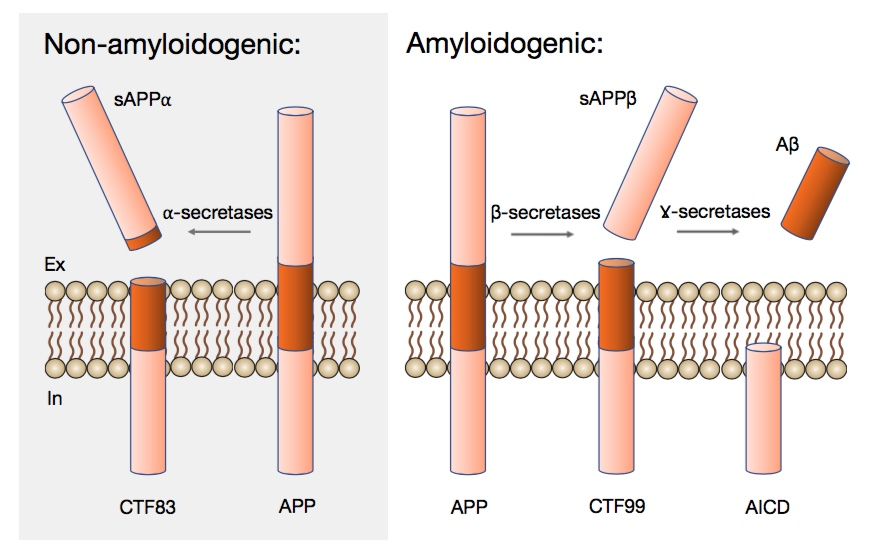
\includegraphics[width=0.8\textwidth]{./Chapter_fly/ab_processing_my_version}
    \caption{%
        Processing pathways of APP.
        Figure adapted from \cite{LaFerla2007}.
    }
    \label{fig:ab_processing}
\end{figure}

\subsubsection{The Arctic mutant}

The Arctic mutation in Aβ42 (Glu22Gly) \cite{Mullan1992} causes a particularly
aggressive form of familial AD that is associated with an increased rate and
volume of plaque deposition \cite{Nilsberth2001}.
Genetic analyses of SAD, however, suggest a complex molecular pathology,
in which alterations in neuro-inflammation, cholesterol metabolism and synaptic recycling
pathways may also be required for Aβ42 to initiate the toxic cascade of events
leading to tau pathology and neuronal damage in dementia.

\subsubsection{Plaque formation}

Late-stage AD brains are characterized by insoluble fibrillar deposits of Aβ,
known as senile plaques.
Plaques are formed in a nucleated event initiated by the pathogenic
Aβ42 peptide \cite{Jarrett1993}.
Aβ can exist in a number of oligomeric states (\ref{fig:ab_states}).
Small oligomers act as nucleation centres that can be elongated into protofibrils.
Ultimately, protofibrils aggregate into larger assemblies known as fibrils.
Subunits of Aβ polymerize by forming β-sheets perpendicular to the protofibril
axis \cite{Serpell2000}.
Monomeric and fibrillar states are innocuous, whilst small oligomers lacking defined
secondary structure are neurotoxic \cite{Ahmed2010}.

Much debate has surrounded the role of Aβ42 in plaque formation because it constitutes just
$10\%$ of the Aβ pool \cite{LaFerla2007}, but dominates plaque composition \cite{Miller1993}.
The first definitive piece of evidence came from a study of mice overexpressing Aβ40 or Aβ42
\cite{McGowan2005}.
Aβ42 was shown to be essential for plaque formation,
whilst plaques do not even form with Aβ40.
But this is not to say that plaques are homogenous.
A proteomics study found that plaques contain on average $913$ proteins,
of which $279$ are consistently found \cite{Drummond2017}.

\begin{figure}[!hbt]
    \centering
    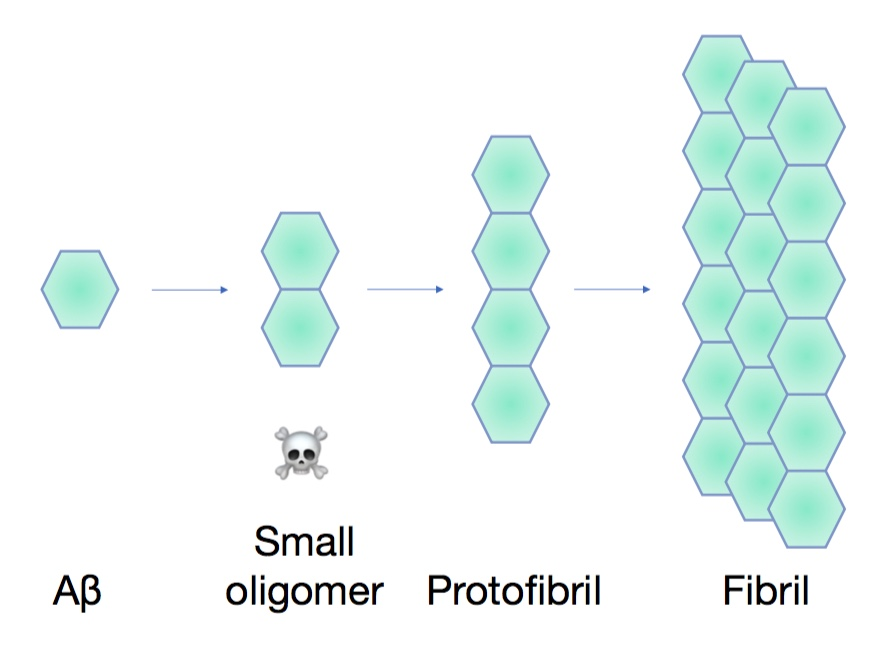
\includegraphics[width=0.5\textwidth]{./Chapter_fly/ab_states_my_version}
    \caption{%
        Oligomeric states of Aβ.
        Figure adapted from \cite{LaFerla2007}.
    }
    \label{fig:ab_states}
\end{figure}

FAD is linked to mutations that lead to increased accumulation of extracellular
Aβ42 \cite{Younkin1998}.
Mutations implicated in FAD have been shown to alter the conformation of Aβ
and affect its aggregation \cite{Hatami2017}.
Of particular interest to this study is the Arctic mutant Aβ42 that is associated with
decreased levels of Aβ in plasma, an increased rate of aggregation
and neurotoxicity \cite{Nilsberth2001,Murakami2002}.

Traditionally, Aβ was thought to only accumulate extracellularly.
Intraneuronal amyloid was first identified by immunohistochemistry \cite{Masters1985}.
More recently, staining with C-terminal specific anti-Aβ antibodies provided evidence
of intraneuronal Aβ42 accumulation prior to the formation of plaques
and neurofibrillary tangles (NFTs) \cite{Gouras2000}.
Indeed, it is believed that intraneuronal Aβ accumulates first and is the source of Aβ
that develops into extracellular plaques \cite{Gouras2000}.
Additionally, intracellular Aβ42 induces cell death by apoptosis,
whereas extracellular Aβ42 and intra-/extracellular Aβ40 are nontoxic \cite{Zhang2002}.
Overall it appears that senile plaques are a marker of advanced AD, whereas,
smaller oligomers of Aβ42 are pathological.

\subsubsection{Involvement of tau}

tau is a neuronal protein that interacts with tubulin to promote
and maintain microtubule assembly \cite{Weingarten1975}.
Intraneuronal aggregates of tau form NFTs in the second AD lesion of AD.
tau is also implicated in a number of other neurological conditions,
known as tauopathies \cite{Iqbal2010}.
A link between Aβ and tau has been established, although there is debate as to the
importance of these agents in AD progression.
Mechanistically, Aβ42 induces the abnormal hyperphosphorylation of tau,
which subsequently form paired helical fragment building blocks of NFTs \cite{Iqbal2010}.
This was confirmed by injecting Aβ42 into the brains of mice,
causing NFTs to form locally \cite{Gotz2001}.
In a similar vain to plaques, whilst NFTs are a hallmark of AD,
they appear to be inert \cite{Alonso2006}.
But $40\%$ of hyperphosphorylated tau is monomeric in AD \cite{Iqbal2010}
and it is this form that is neurotoxic, sequesters normal tau
and promotes the disassembly of microtubules \cite{Alonso1994}.
In summary, soluble Aβ and tau work in conjunction to convert healthy neurons into
a diseased state, occurring independently of plaques and NFTs.

\subsubsection{Proteomics}

Post-mortem proteomics studies on human brains have been valuable in adapting the amyloid cascade hypothesis of AD and helped develop the alternative neuro-inflammation hypothesis of AD.
These studies revealed that the brain undergoes oxidative damage as a response to amyloid accumulation in the end stages of disease.
Using model organisms, such as fruit flies, allows molecular alterations in the brain to be tracked from the onset of AD, during its progression, until death.
Comparison of proteomic analyses of post-mortem human brains have further revealed an increase in metabolic processes and reduction in synaptic function in AD \cite{Moya-Alvarado2016}.
Oxidised proteins also accumulate at early stages in AD brain, probably as a result of mitochondrial ROS production \cite{Lynn2010}, and redox proteomic approaches suggest that enzymes involved in glucose metabolism are oxidised in mild cognitive impairment and AD \cite{Butterfield2014,Aluise2011}.
Moreover, phospho-proteomic approaches have revealed alterations in phosphorylation of metabolic enzymes and kinases that regulate phosphorylation of chaperones such as HSP27 and crystallin alpha B \cite{Dammer2015}.
Of note, however, there is little proteomic overlap between studies using post-mortem human brain tissue, which may reflect the low sample numbers available for such studies, differences in comorbidities between patients and confounding post-mortem procedures \cite{Moya-Alvarado2016}.
Although valuable, post-mortem studies also reflect the end-stage of disease and, therefore, do not facilitate measurement of dynamic alterations in proteins as AD progresses.

\subsubsection{Animal models}

Animal models of AD, generated through transgenic over-expression of human APP or tau, provide an opportunity to track proteomic alterations at pre- and post-pathological stages, thus facilitating insight into the molecular mechanisms underlying disease development and revealing new targets for drugs to prevent AD progression.
Analyses of transgenic mice models of AD have revealed some overlapping alterations in metabolic enzymes, kinases and chaperones with human AD brain \cite{Moya-Alvarado2016}.
Only one study, however, has tracked alterations in protein carbonylation over time, showing increases in oxidation of metabolic enzymes (alpha-enolase, ATP synthase $\alpha$-chain and pyruvate dehydrogenase E1) and regulatory molecules (14-3-3 and Pin1) in correlation with disease progression \cite{Sultana2011}.

Adult-onset \textit{Drosophila} models of AD have been generated by over-expressing human Aβ42 peptide exclusively in adult fly neurons using inducible expression systems.
These models have been shown to develop progressive neurodegenerative phenotypes, such as reduced climbing ability, and shortened lifespan \cite{Sofola2010}.
Taking advantage of the short lifespan of the fly, and the flexible nature of the inducible model, we have performed a longitudinal study of the brain proteome to capture the effects of Aβ42-toxicity in the brain from the point of induction and across life.


\subsection{Mass spectrometry}

Mass spectrometry (MS) is a sensitive analytical technique that was developed in 1912.
MS measures the mass-to-charge ratio ($m/z$) of an analyte.
Over the past century, MS has seen rapid development and has created many distinct, but related, fields.
This is largely due to MS being able to measure the $m/z$ of analytes whose masses range over several orders of magnitude---from small molecules under $100$ Da to a $52$ MDa whole virus \cite{Keifer2016}.

There are three main components in any mass spectrometer: the source, analyser and detector.
Analyte molecules are ionised to form positive ions by the source.
Many different types of source have been developed, including soft and hard ionisation methods, some of which are covered below.
All ions with the same charge are then accelerated to the same kinetic energy ($KE = \frac{mv^2}{2}$).
By rearranging the equation, we find that the velocity of an ion depends on its mass ($v = \sqrt{\frac{2KE}{m}}$), so heavier ions will have a lower velocity than lighter ions.
Analysers exploit this property to sort ions according to $m/z$.
For example, time-of-flight analysers accelerate ions through a flight tube and measure the $m/z$ by the time it takes for the ion to reach the detector.
Finally, any ions that pass through the analyser are detected as an electrical current by the negatively charged detector.

One such burgeoning MS field is proteomics---the study of proteomes by MS \cite{Wasinger1995,Aebersold2003}.
Technological developments in MS that are relevant to proteomics---and particularly the methods used in this study---are introduced below.

\subsubsection{Soft ionisation}

Traditional electron ionisation methods use an electron beam to form positive ions by knocking elctrons off molecules.
This method is high-energy and leads to fragmentation of molecules, so is unsuitable for the analysis of proteins.
Two soft ionisation methods were developed in the 1980s, which allowed MS to be applied to macromolecules with minimal fragmentation.
Matrix-assisted laser desorption/ionisation (MALDI) uses a laser to liberate the analyte from a laser-absorbing matrix \cite{Tanaka1988,Karas1985}.
Electrospray ionisation (ESI) applies a high voltage to a liquid containing the analyte, which produces an aerosol \cite{Whitehouse1985}.
Unlike MALDI, ESI is able to create multiply charged ions, which extends the $m/z$ range that can be detected.
In 2002, the inventors of these methods were awarded The Nobel Prize in Chemistry.

\subsubsection{Ion-mobility}

Ion-mobility spectrometry is a method of separating ions in the gas phase \cite{Gabelica2018}.
Ions enter a drift tube that is filled with a buffer gas and are moved through the drift tube with an electric field.
Particles of the buffer gas collide with the ions, which creates a frictional force that impedes their progress.
The time that it takes for a molecule to move through the drift tube is known as the arrival time.
The rate of these collisions depends on the ion's collision cross section (CCS), a measure that quantifies the overall shape of a particle.
CCS refers to the ensemble of all possible geometric orientations of a particle, and all possible interaction types that it may have with other particles in the gas phase, averaged into a cross sectional area of a circle \cite{May2017}.
Although the CCS of a protein is correlated with its mass, there is a high variance in CCS for any given mass \cite{May2017}.
This makes intuitive sense because proteins are not perfect spheres of uniform density---some are elongated and others have pockets.
CCS predicts that spheroidal globular proteins will collide less often with the buffer gas than proteins with a large surface area-to-volume ratio.
Furthermore, chemically identical protein molecules do not have exactly the same arrival time, but rather their arrival times are distributed, due to conformational differences.
Differential CCS allows ions to be separated by their arrival time an additional dimension of shape, thus enabling ion-mobility spectrometers to separate ions according to their arrival time, which depends on the $m/z$ and shape of the particle.
Abstractly, ion-mobility is somewhat similar to gel filtration chromatography, in that proteins are separated by their shape.
Both CCS and arrival time are not inherent properties of particles because they depend on the buffer gas used and the temperature \cite{Gabelica2018}.

\subsubsection{Tandem mass spectrometry}

MS-based proteomics typically uses a tandem MS (MS/MS) setup, consisting of MS1 and MS2 stages \cite{Schubert2017}.
Proteins with a particular $m/z$ are selected in MS1 using an analyser, such as an ion-mobility, time-of-flight or quadrupole analyser.
The protein is then fragmented in MS2 and the resulting peptides are detected.
The combination of the fragment ion's mass spectrum and $m/z$ are sufficient to determine its amino acid sequence \cite{Noor2019}.

To further improve the performance of MS/MS for proteomics, proteins are first purified by liquid chromatography, so called LC-MS/MS \cite{Henderson1992}.
Liquid chromatography separates proteins by some property, such as size in gel filtration, or polarity in high performance liquid chromatography (HPLC) and ultra performance liquid chromatography (UPLC), due to differences in how proteins in the sample interact with the mobile and stationary phases.
Proteins are eluted from chromatography columns and the eluent is directly analysed by the MS instrument.
We used a reverse phase UPLC column in this study.
Typically HPLC and UPLC use a normal phase column that has a polar stationary phase.
Polar molecules will interact more strongly with the stationary phase and will elute slowly, whereas, non-polar molecules will interact weakly and will elute quickly.
In reverse phase columns, the stationary phase is non-polar, so the situation is reversed and non-polar molecules interact strongly and elute slowly.

We used a Waters Synapt GS-Si tandem mass spectrometer in this study (\ref{fig:synapt}).
This instrument uses a quadrupole, followed by an ion-mobility analyser for MS1 and a time-of-flight analyser for MS2.

\begin{figure}[!hbt]
    \centering
    \ifredact
        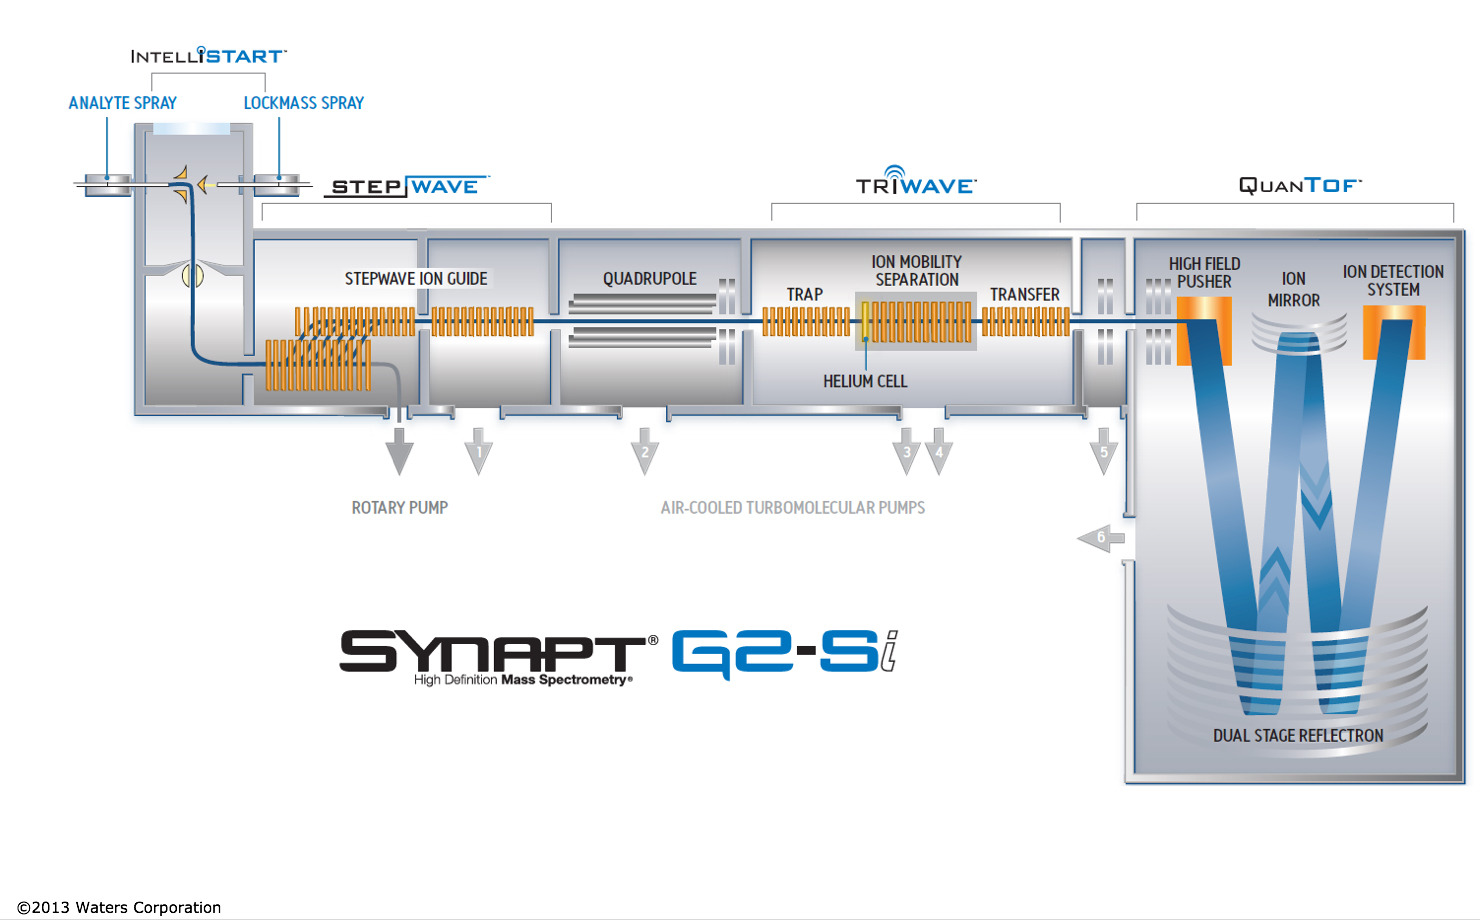
\includegraphics[draft=true, width=\textwidth, trim={0 5cm 0 0}, clip]{./Chapter_fly/synapt}
    \else
        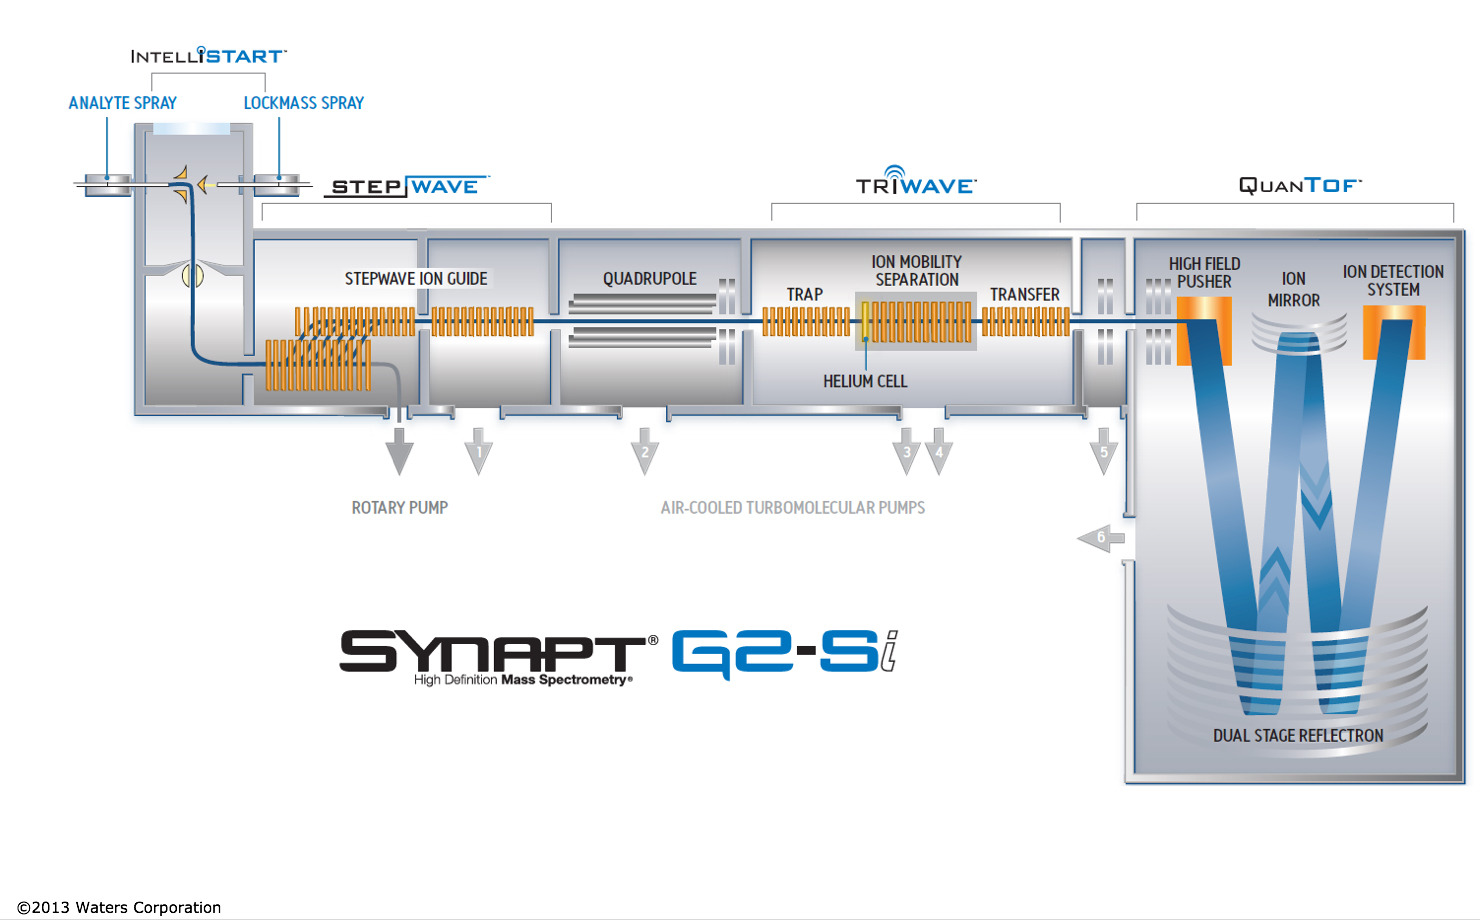
\includegraphics[width=\textwidth, trim={0 5cm 0 0}, clip]{./Chapter_fly/synapt}
    \fi
    \caption{%
        Schematic of the Synapt GS-Si mass spectrometer.
        Figure produced by Waters Corporation.
    }
    \label{fig:synapt}
\end{figure}

\subsubsection{Quantitative label-free proteomics}

The intensity of electric current that is generated by fragment ions in MS2 can be used to estimate the relative abundance of the protein in the sample \cite{Schubert2017}.
So that abundances can be compared across multiple samples, relative abundances are normalised to a reference peptide that is spiked-in at known concentration and converted to meaningful units.
Sample preparations for label-free MS is simpler than labeled methods, but label-based methods remain the most accurate methods for quantification.

\subsubsection{Data-independent acquisition}

Data-independent acquisition (DIA) is a high-throughput and unbiased method of acquiring MS data \cite{Gillet2016,Chapman2014}.
Prior to the advent of DIA, data-dependent acquisiton was used, which is low-throughput.
In DIA, the entire $m/z$ range is analysed by fragmenting all ions, or predefined $m/z$ windows.
If samples are complex, then the peptides that are detected will be highly multiplexed, requiring software analysis tools to deconvolute the data.
Modern DIA methods use ion-mobility \cite{Geromanos2012}.

\subsection{Contributions}

AD, the most prevalent form of dementia,
is a progressive and devastating neurodegenerative condition for which
there are no effective treatments.
Understanding the molecular pathology of AD during disease progression may identify
new ways to reduce neuronal damage.
Here, we present a longitudinal study tracking dynamic proteomic alterations in the brains
of an inducible \textit{Drosophila melanogaster} model of AD expressing the Arctic mutant Aβ42 gene.
We identified $3093$ proteins from flies that were induced to express Aβ42
and age-matched healthy controls
using label-free quantitative ion-mobility data independent analysis mass spectrometry.
Of these, $228$ proteins were significantly altered by Aβ42 accumulation
and were enriched for AD-associated processes.
Network analyses further revealed that these proteins have distinct hub
and bottleneck properties in the brain protein interaction network,
suggesting that several may have significant effects on brain function.
Our unbiased analysis provides useful insights into the key processes governing
the progression of amyloid toxicity and forms a basis for further functional analyses
in model organisms and translation to mammalian systems.

\section{Methods}
\label{methods}

\subsection{Data collection}

\subsubsection{Fly stocks}

The transgenic AD (TgAD) fly line used in this study \cite{Sofola2010} contains the human transgene encoding the Arctic mutant Aβ42 peptide under the control of an Upstream Activation Sequence (UAS) \cite{Crowther2005}.
Expression of Aβ42 was controlled by GeneSwitch \cite{Osterwalder2001}---a mifepristone-inducible GAL4/UAS expression system---under the pan-neuronal elav promoter.
All flies were backcrossed for six generations into the w$^{1118}$ genetic background.

Flies were grown in $200$ ml bottles on a $12$ h/$12$ h light/dark cycle at constant temperature ($25$$^{\circ}$C) and humidity.
Growth media contained $15$ g/l agar, $50$ g/l sugar, $100$ g/l autolysed yeast, $100$ g/l nipagin and $3$ ml/l propionic acid.
Flies were maintained for two days after eclosion before females were transferred to vials at a density of $25$ flies per vial for the lifespan analysis and $10$ flies per vial for the IM-DIA-MS analysis.
Expression of Aβ42 was induced in TgAD flies by spiking the growth media with mifepristone to a final concentration of $200$ µM.
Flies were transferred to fresh media three times per week, at which point the number of surviving flies was recorded.
For each of the three biological repeats, $10$ healthy and $10$ Aβ42 flies were collected at $5$, $19$, $31$ and $46$ days, as well as $54$ and $80$ days for healthy flies.
Following anesthetisation with CO\textsubscript{2}, brains were dissected in ice cold $10$ mM phosphate buffered saline snap frozen and stored at $-80$$^{\circ}$C.

\subsubsection{Extraction of brain proteins}

Brain proteins were extracted by homogenisation on ice into $50$ µl of $50$ mM ammonium bicarbonate, $10$ mM DTT and $0.25\%$ RapiGest detergent.
Proteins were solubilised and disulfide bonds were reduced by heating at $80$$^{\circ}$C for $20$ minutes.
Free cysteine thiols were alkylated by adding $20$ mM IAA and incubating at room temperature for $20$ minutes in darkness.
Protein concentration was determined and samples were diluted to a final concentration of $0.1\%$ RapiGest using $50$ mM ammonium bicarbonate.
Proteins were digested with trypsin overnight at $37$$^{\circ}$C at a $50:1$ protein:trypsin ratio.
Additional trypsin was added at a $100:1$ ratio the following morning and incubated for a further hour.
Detergent was removed by incubating at $60$$^{\circ}$C for one hour in $0.1\%$ formic acid.
Insoluble debris was removed by centrifugation at \num{14000}x g for $30$ minutes.
Supernatant was collected, lyophilised and stored at $-80$$^{\circ}$C.
Prior to lyophilisation peptide concentration was estimated by nanodrop (Thermo Fisher Scientific, Waltham, MA).

\subsection{Label-free quantitative IM-DIA-MS}

Peptides were separated by nanoscale liquid chromatography (LC) by loading $300$ ng of protein onto an analytical reversed phase column.
IM-DIA-MS analysis was performed using a Synapt G2-Si mass spectrometer (Waters Corporation, Manchester, UK).
The time-of-flight analyzer of the instrument was externally calibrated with a NaCsI mixture from $m/z$ \numrange{50}{1990}.
Spectra were acquired over a range of \numrange{50}{2000} $m/z$. Each biological repeat was analysed at least twice to account for technical variation.
LC-MS data were peak detected and aligned by Progenesis QI for proteomics (Waters Corporation).
The principles of the embedded search algorithm for DIA data has been described previously \cite{Li2009}.
Proteins were identified by searching against the \textit{Drosophila melanogaster} proteome in UniProt, appended with common contaminants, and reversed sequence entries to estimate protein identification false discovery rate (FDR) values, using previously specified search criteria \cite{Distler2014}.
Peptide intensities were normalised to control for variation in protein loading and relative quantification.
Abundances were estimated by Hi3-based quantitation \cite{Silva2006}.

\subsubsection{IM-DIA-MS analysis}

Nanoscale LC separation of tryptic peptides was performed using a nanoAcquity UPLC system (Waters Corporation) equipped with a UPLC HSS T3 $1.7$ µm, $75$ µm x $250$ mm analytical reverse phase column (Waters Corporation).
Prior to peptide separation, $300$ ng of tryptic peptides were loaded onto a 2G, V/V 5 µm, $180$ µm x $20$ mm reverse phase trapping column at $5$ µl/min for three minutes.
IM-DIA-MS analysis of tryptic digests was performed using a Synapt GS-Si mass spectrometer equipped with a T-Wave-IMS device.
Mass measurements were made in positive-mode ESI with the instrument operated in resolution mode with a typical resolving power of \num{20000} full width at half maximum.
Prior to analysis the time-of-flight analyzer was externally calibrated with a NaCsI mixture from $m/z$ \numrange{50}{1990}. The data were post-acquisition lock mass corrected using the double charged monoisotopic ion of [Glu1]-Fibrinopeptide B.
To achieve lock mass correction, a $100$ fmol/µl solution of [Glu1]-Fibrinopeptide B was infused at a $90$° angle to the analytical sprayer. This reference sprayer was sampled every $60$ seconds.
Accurate IM-DIA-MS data were collected in the DIA mode of analysis, HDMS\textsuperscript{E} IM spectrometry was performed by applying a constant wave height of $40$ V whilst a constant wave velocity of 650 m/s was maintained.
Wave heights within the trap and transfer were both set at $4$ V whilst the wave velocities were $311$ and $175$ m/s respectively.
MS data were acquired over \numrange{50}{2000} $m/z$ for each mode.
Spectral acquisition time for each mode was $0.5$ s with a $0.015$ interscan delay, corresponding to a cycle of low and elevated energy data being acquired every $1.1$ s.
During the low energy MS mode data was acquired whilst applying a constant collision energy of $4$ eV within the transfer.
After IMS, MS/MS data was acquired by ramping the collision energy within the transfer region between $15$ and $45$ eV.
To ensure that ions with a $m/z$ less than $350$ were derived from peptide fragmentation within the transfer region the radio frequency applied to the quadrupole mass analyser was adjusted to optimise transmission within the region of \numrange{350}{2000} Da.
Each biological replicate was analysed at least twice.

\subsubsection{MS Data Processing}

All MS data were processed in Progenesis QI for proteomics.
Data were imported into Progenesis to generate a $3$D representation of the data ($m/z$, retention time and peak intensity).
Samples were then time aligned with the software allowed to automatically determine the best reference run from the dataset.
Following alignment, peak picking was performed on MS level data. A peak picking sensitivity of $4$ (out of $5$) was set.
Peptide features were tentatively aligned with their respective fragment ions based primarily on the similarity of their chromatographic and mobility profiles.
Requirements for features to be included in post-processing database searching were as follows: $300$ counts for low energy ions, $50$ counts for high energy ions and $750$ counts for deconvoluted precursor intensities.
Subsequent data were searched against \num{20049} sequences from the UniProt canonical \textit{Drosophila} database (appended with common contaminants).
Trypsin was specified as the enzyme of choice and a maximum of two missed cleavages were permitted.
Carbamidomethyl (C) was set as a fixed modification whilst oxidation (M) and N-terminal acetylation were set as variable modifications.
Peptide identifications were grouped and relative quantification was performed using non-conflicting peptides only.

\subsection{Data analysis}

\subsubsection{Data processing}

Proteins that were identified in both healthy and Aβ42 flies were considered for further analysis.
Missing data were replaced by the minimum abundance measured for any protein in the same repeat \cite{Lazar2016a}.
The data were quantile normalised \cite{Bolstad2003}, so that different conditions and time points could be compared reliably.
Quantile normalisation transforms the abundances so that each repeat has the same distribution.

For principal component analysis (PCA) analysis, the data were $\log_{10}$-transformed and each protein was standardised to zero mean and unit variance.
Hierarchical biclustering was performed using the Euclidean distance metric with the complete linkage method.
Prior to clustering, proteins were normalised to their abundance in healthy flies at $5$ days.

Proteins that were identified by IM-DIA-MS in either healthy or Aβ42 flies were assessed for overrepresentation of Gene Ontology (GO) terms using GOrilla \cite{Bolstad2003}, which uses ranked lists of target and background genes.
Proteins were ranked in descending order by their mean abundance. The type I error rate was controlled by correcting for multiple testing using the Benjamini-Hochberg method at an FDR of $5\%$.
Clusters of proteins were assessed for overrepresentation of GO-Slim terms in the Biological Process ontology using Panther (version 13.1) with a custom background of the \num{3093} proteins identified by IM-DIA-MS in healthy or AD flies.

\subsubsection{Identification of significantly altered proteins}

Significantly altered proteins were identified using five methods that are frequently used to identify differentially expressed genes in time course RNA-Seq data.
DESeq2 \cite{Love2014}, EDGE \cite{Woo2011}, edgeR \cite{Robinson2010}, limma \cite{Ritchie2015} and maSigPro \cite{Nueda2014} are all available in R through Bioconductor.
Dispersions were estimated from the biological and technical repeats. Unless otherwise stated, default parameters were used for all methods under the null hypothesis that a protein does not change in abundance between healthy and AD conditions in normal ageing.
The type I error rate was controlled by correcting for multiple testing using the Benjamini-Hochberg method at a FDR of $5\%$.
A protein was classified as significantly altered if two or more methods identified it.

DESeq2 models proteins with the negative binomial distribution and performs likelihood ratio tests.
A time course experiment was selected in EDGE using the likelihood ratio test and a normal null distribution.
edgeR uses the negative binomial distribution and performs quasi-likelihood tests.
limma fits linear models to the proteins and performed empirical Bayes F-tests.
maSigPro fits generalised linear models to the proteins and performs log-likelihood ratio tests.

Significantly altered proteins were clustered using a Gaussian mixture model.
Protein abundances were $\log_{10}$-transformed and $z$ scores were calculated.
Gaussian mixture models were implemented for \numrange{1}{228} clusters.
The best model was chosen using the Bayesian information criterion (BIC), which penalises complex models $\text{BIC} = -2 \ln(L) + \ln(n)k$, where $\ln(L)$ is the log-likelihood of the model, $n$ is the number of significantly altered proteins and $k$ is the number of clusters.
The model with lowest BIC was chosen.

\subsubsection{Networks}
\label{sec:fly-networks-methods}

All network analysis was performed using the \textit{Drosophila melanogaster} Search Tool for the Retrieval of Interacting Genes/Proteins (STRING) network (version 10) \cite{Szklarczyk2015}.
Low confidence interactions with a `combined score' $< 0.5$ were removed in all network analyses.

Network properties of the significantly altered proteins were analysed in the brain protein interaction network.
A subgraph of the STRING network was induced on the \num{3093} proteins identified by IM-DIA-MS in healthy or Aβ42 flies and the largest connected component was selected (\num{2428} nodes and \num{44561} edges).
The subgraph contained $183$ of the $228$ significantly altered proteins.
% (\ref{fig:fly-figS6}
%; Supplementary Data 4
%)
For these proteins, four network properties were calculated as test statistics: mean node degree; mean unweighted shortest path length between a node and the remaining $182$ nodes; the size of the largest connected component in the subgraph induced on these nodes; and mean betweenness centrality.
Hypothesis testing was performed using the null hypothesis that there is no difference between the nodes in the subgraph.
Assuming the null hypothesis is true, null distributions of each test statistic were simulated by randomly sampling $183$ nodes from the network \num{10000} times.
Using the null distributions, one-sided non-parametric $P$ values were calculated as the probability of observing a test statistic as extreme as the test statistic for the significantly altered proteins.

A subgraph of the STRING network was induced on the proteins significantly altered in AD and their neighbours and the largest connected component was selected (\num{4842} nodes and \num{182474} edges).
The subgraph contained $198$ of the $228$ significantly altered proteins and was assessed for enrichment of GO terms. Densely connected subgraphs were identified using MCODE \cite{Bader2003}.
Modules were selected with an MCODE score $> 10$. As STRING is a functional interaction network, clusters of nodes may correspond to proteins from the same complex, pathway or functional family.
Clusters were assessed for overrepresentation of GO Slim terms in the Biological Process ontology using Panther \cite{Mi2013} (version 13.1) with a custom background of the \num{3093} proteins identified by IM-DIA-MS in healthy or Aβ42 flies.
Fisher’s exact tests were performed and the type I error rate was controlled by correcting for multiple testing using the Benjamini-Hochberg method at an FDR of $5\%$.

\subsubsection{Open source software}

Data analysis was performed in Python v3.6 (Python Software Foundation, http://\-www.\-python.org) using SciPy \cite{Oliphant2007}, NumPy \cite{Oliphant2006}, Pandas \cite{McKinney2010}, scikit-learn \cite{Pedregosa2011}, NetworkX \cite{Hagberg2008}, IPython \cite{Perez2007} and Jupyter \cite{Kluyver2016}.
Figures were plotted using Matplotlib \cite{Hunter2007} and seaborn.

\section{Results}
\label{results}

\subsection{Proteome analysis of healthy and Aβ42-expressing fly brains}

In this study, we used an inducible transgenic fly line expressing human Arctic mutant Aβ42 (TgAD) \cite{Crowther2005,Osterwalder2001} (\ref{fig:fly-fig1}a).
Flies were either chronically induced two days after eclosion (Aβ42 flies) or remained uninduced (healthy flies) and used as a control of normal ageing.

We first sought to determine how the fly lifespan is affected in TgAD.
We confirmed a previously observed \cite{Sofola2010} reduction in lifespan following
Aβ42 induction prior to proteomic analyses (\ref{fig:fly-fig1}b).

%, Supplementary Data 1
To understand how the brain proteome is affected as Aβ42 toxicity progresses,
fly brains were dissected from healthy and Aβ42 flies at $5$, $19$, $31$ and $46$ days,
and at $54$ and $80$ days for healthy controls,
then analysed by label-free quantitative IM-DIA-MS (\ref{fig:fly-fig1}c).
\num{1854} proteins were identified in both healthy and Aβ42 fly brain from a total of
\num{3093} proteins (\ref{fig:fly-fig1}d),
which is typical for recent fly proteomics studies \cite{Brown2018,Tain2017}.

\clearpage

\begin{figure}[hp!]
    \centering
    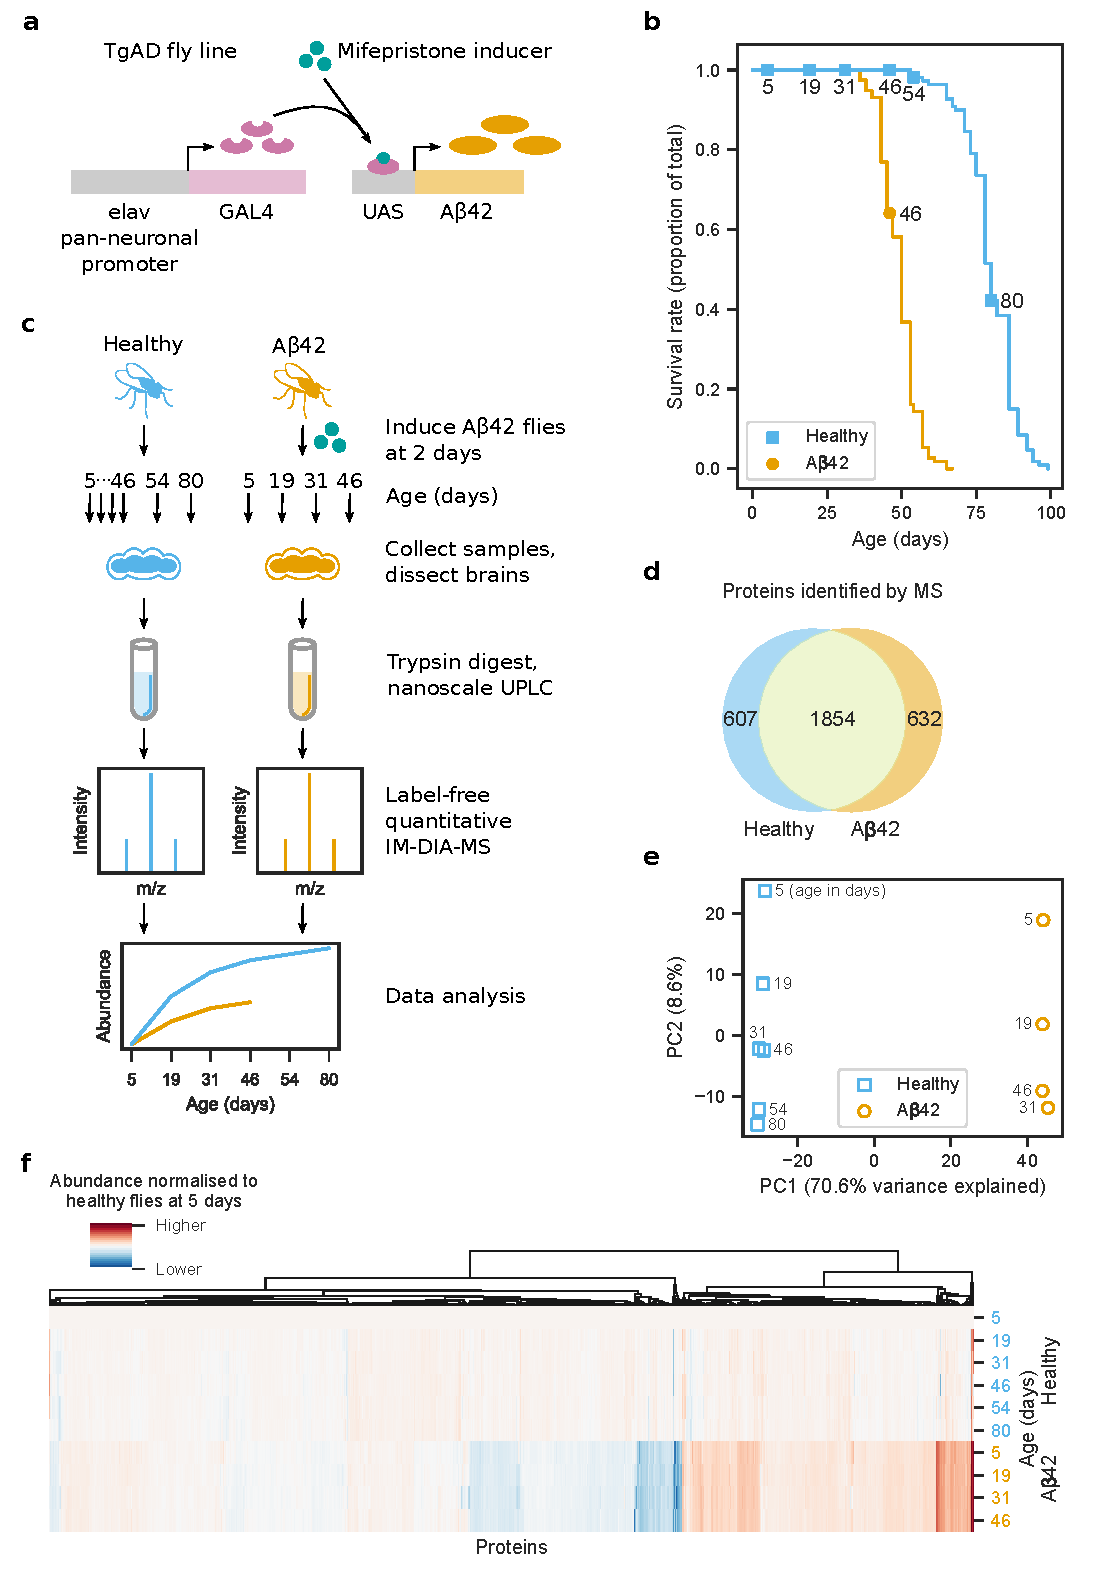
\includegraphics[width=1.1\textwidth]{./Chapter_fly/fig1}
    \caption{%
        Proteome analysis of healthy and AD fly brains.
        \textit{Cont}.
    }
    \label{fig:fly-fig1}
\end{figure}

% caption continues on the next page
\clearpage
\addtocounter{figure}{-1}

\begin{center}
    \captionsetup{type=figure,list=no} % Do not add continued caption to the LOF
    \captionof{figure}{%
        Proteome analysis of healthy and AD fly brains.
        (a) \textit{Drosophila melanogaster} transgenic model of AD (TgAD) that expresses Arctic mutant Aβ42 in a mifepristone-inducible GAL4/UAS expression system under the pan-neuronal elav promoter.
        (b) Survival curves for healthy and Aβ42 flies.
        Aβ42 flies were induced to express Aβ42 at $2$ days.
        Markers indicate days that MS samples were collected.
        (c) Experimental design of the brain proteome analysis.
        Aβ42 flies were induced to express Aβ42 at $2$ days.
        For each of the three biological repeats, $10$ healthy and $10$ Aβ42 flies were collected at $5$, $19$, $31$ and $46$ days,
        and at $54$ and $80$ days for healthy controls.
        Proteins were extracted from dissected brains and digested with trypsin.
        The resulting peptides were separated by nanoscale liquid chromatography and analysed by label-free quantitative IM-DIA-MS.
        (d) Proteins identified by IM-DIA-MS.
        (e) Principal component analysis of the IM-DIA-MS data.
        Axes are annotated with the percentage of variance explained by each principal component.
        (f) Hierarchical biclustering using relative protein abundances normalised to their abundance in healthy flies at $5$ days.
    }
\end{center}

%(\ref{fig:fly-figS1}).
For the \num{1854} proteins identified in both healthy and Aβ42 flies,
we assessed the reliability of our data.
Proteins were highly correlated between technical and biological repeats
We used principal component analysis of the protein abundances
to identify sources of variance (\ref{fig:fly-fig1}e).
Healthy and Aβ42 samples are clearly separated in the first principal component,
probably due to the effects of Aβ42.
In the second principal component, samples are separated by increasing age,
due to age-dependent or disease progression changes in the proteome.
These results show that whilst ageing does contribute to changes in the brain proteome
($8.7\%$ of the total variance), much larger changes are due to expression of Aβ42 ($70.6\%$)
and this may reflect either a correlation with the ageing process or progression of AD pathology.
We confirmed this result using hierarchical biclustering of protein abundances
in Aβ42 versus healthy flies at $5$ days (\ref{fig:fly-fig1}f).
The results reveal that most proteins do not vary significantly in abundance with age
in healthy flies, but many proteins are differentially abundant in Aβ42 flies.

% \begin{figure}[!hbtp]
%     \centering
%     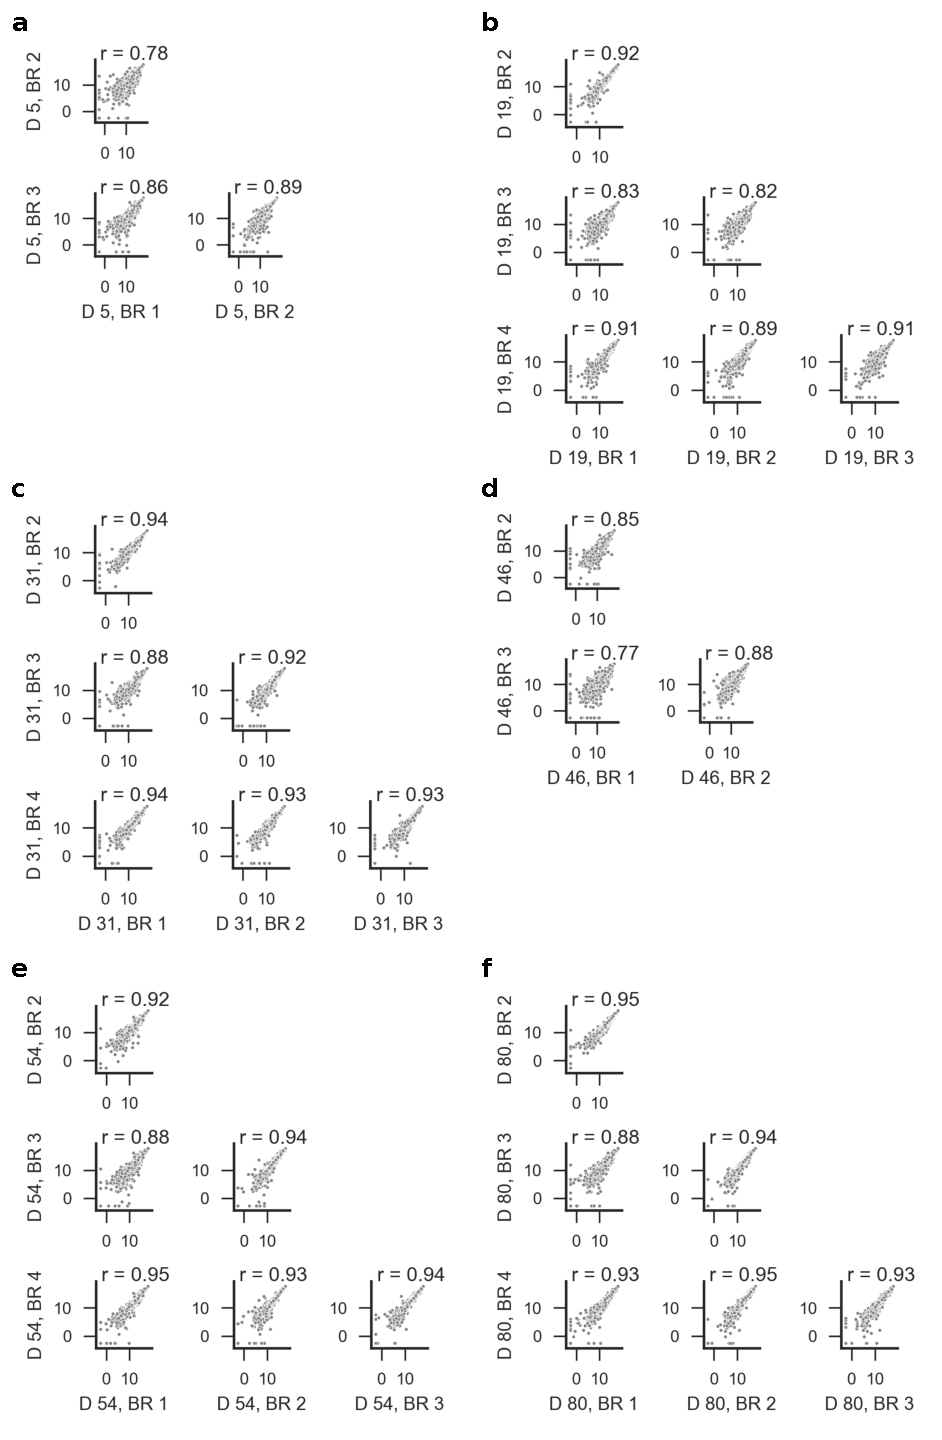
\includegraphics[width=0.8\textwidth]{./Chapter_fly/figS1}
%     \caption{%
%         Assessment of experimental reproducibility.
%         Scatter plots comparing protein abundances in different biological repeats (BR)
%         of healthy flies at days (D) (a) 5, (b) 19, (c) 31, (d) 46, (e) 54 and (f) 80.
%         Abundances were log2-transformed before plotting.
%         Pearson correlation coefficients (r) are shown for each pair of
%         biological repeat at each time point.
%     }
%     \label{fig:fly-figS1}
% \end{figure}

\subsection{Analysis of brain proteome dysregulation in Aβ42 flies}

%; Supplementary Data 2
We next identified the proteins that were significantly altered following Aβ42 expression
in the fly brain.
To achieve this, we used five methods commonly used to analyse time course RNA-Seq data
\cite{Anders2010} and classified proteins as significantly altered if at least
two methods detected them \cite{Zhang2014a}.
We identified $228$ significantly altered proteins from $740$ proteins that were detected
by one or more methods (\ref{fig:fly-fig2}a).
A comparison of popular RNA-Seq analysis tools \cite{Seyednasrollah2015} showed that edgeR
\cite{Robinson2010} has a high false positive rate and variable performance on
different data sets, whereas, DESeq2 \cite{Love2014} and limma \cite{Ritchie2015}
have low false positive rates and perform more consistently.
We observed a similar trend in our data set.
limma and DESeq2 detected the lowest number of proteins, with $21$ proteins
in common (\ref{fig:fly-figS2}a).
edgeR detected more proteins, of which $38$ were also detected by DESeq2 and $16$ by limma.
EDGE \cite{Woo2011} and maSigPro \cite{Nueda2014} detected vastly more proteins,
$464$ of which were only detected by one method.
Principal component analysis shows that edgeR, DESeq2 and limma detect similar proteins,
whereas, EDGE and maSigPro detect very different proteins (\ref{fig:fly-figS2}b).

\begin{figure}[!hbt]
    \centering
    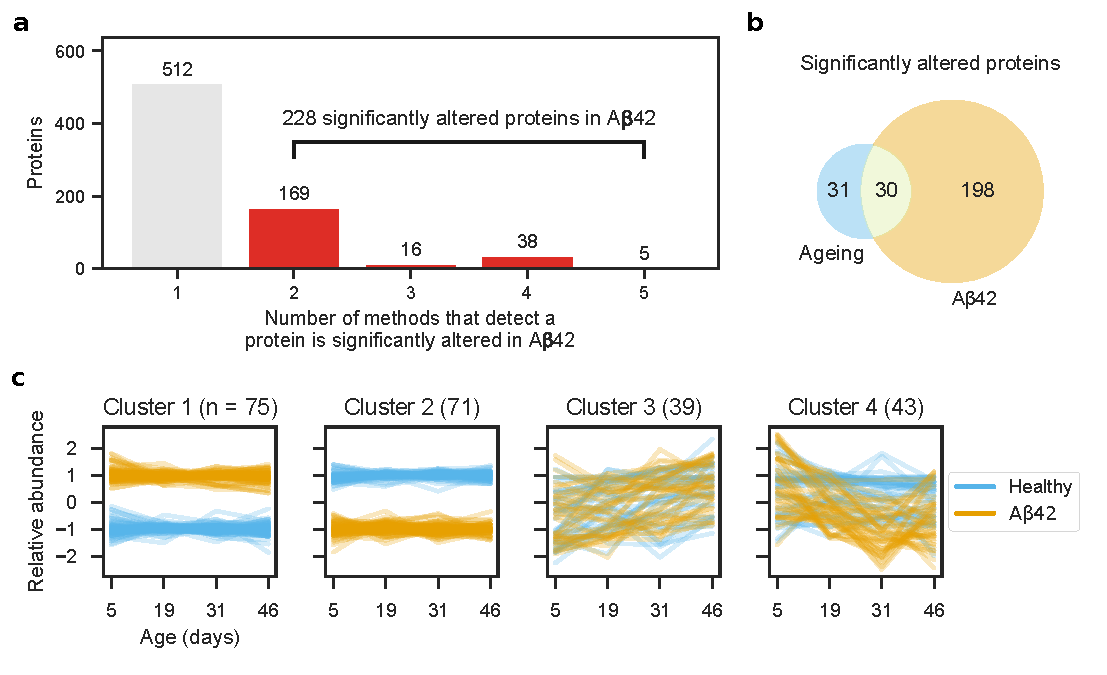
\includegraphics[width=1.05\textwidth]{./Chapter_fly/fig2}
    \caption{%
        Brain proteome dysregulation in AD.
        (a) Proteins significantly altered in AD were identified using five methods
        (EDGE, edgeR, DESeq2, limma and maSigPro) and classified as significantly altered
        if at least two methods detected them.
        (b) Significantly altered proteins in AD (from a) and ageing.
        (c) Significantly altered protein abundances were $z$ score-transformed and
        clustered using a Gaussian mixture model.
    }
    \label{fig:fly-fig2}
\end{figure}

\begin{figure}[!hbt]
    \centering
    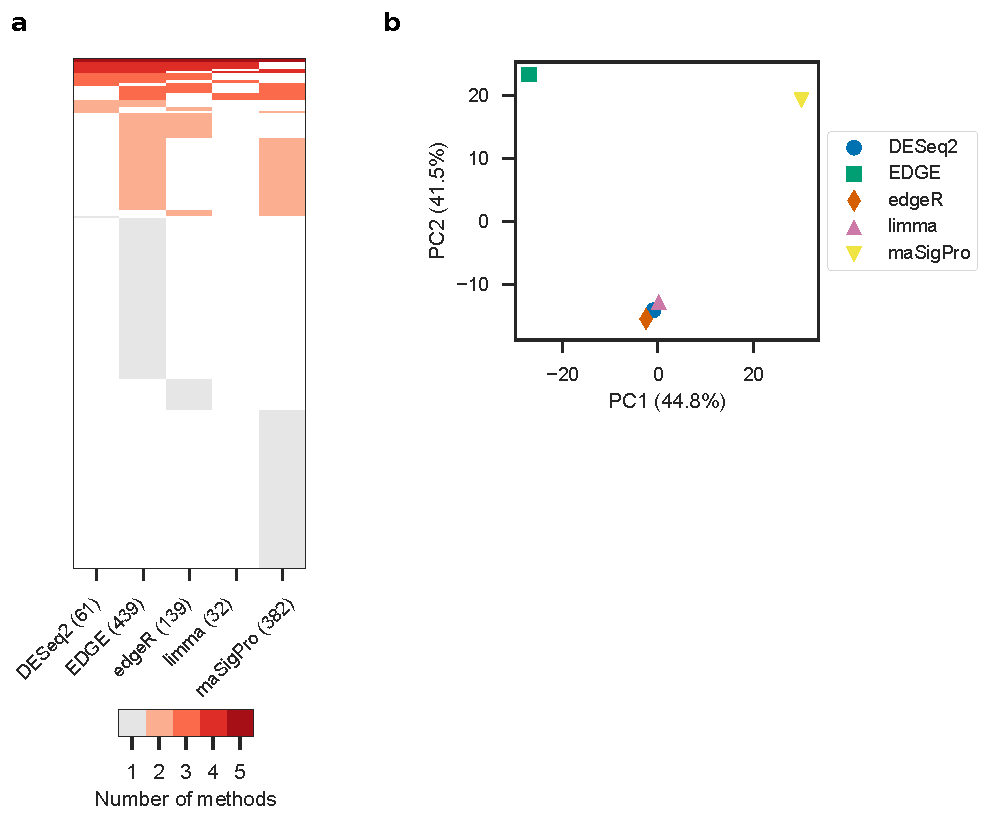
\includegraphics[width=\textwidth]{./Chapter_fly/figS2}
    \caption{%
        Analysis of the five statistical methods used to identify significantly altered proteins.
        (a) Heat map of the proteins detected by each method.
        (b) Principal component analysis of these results.
        Axes are annotated with the percentage of variance explained by each principal component.
    }
    \label{fig:fly-figS2}
\end{figure}

% (\ref{fig:fly-figS3}
%; Supplementary Data 3)

Although these methods should be able to differentiate between proteins that are altered in
Aβ42 flies from those that change during normal ageing,
we confirmed this by analysing healthy flies separately.
In total, $61$ proteins were identified as significantly altered with age,
of which $30$ were also identified
as significantly altered in AD (\ref{fig:fly-fig2}b) and $31$ in normal ageing alone.
These proteins are not significantly enriched for any pathways or functions.
Based on our results, we concluded that the vast majority of proteins
that are significantly altered in AD are not altered in normal ageing
and that AD causes significant dysregulation of the brain proteome.

% \begin{figure}[!hbt]
%     \centering
%     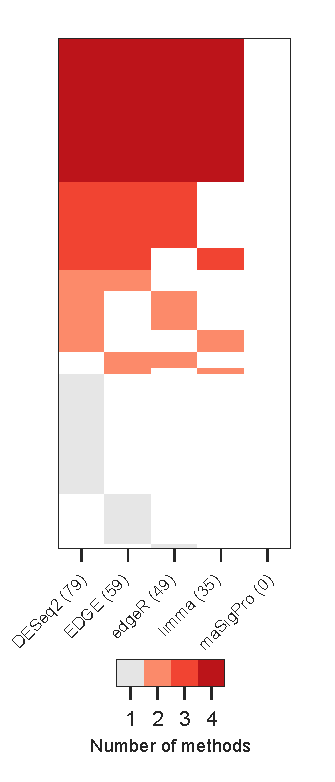
\includegraphics[width=0.4\textwidth]{./Chapter_fly/figS3}
%     \caption{%
%         Identification of significantly altered proteins during normal ageing.
%         Heat map of the proteins detected by each method.
%     }
%     \label{fig:fly-figS3}
% \end{figure}

% (\ref{fig:fly-figS4})
Of the $31$ proteins specifically altered in ageing,
$10$ decreased with age (Acp1, CG7203, mRPL12, qm, CG11017, HIP, HIP-R, PP02 and Rpn1),
$15$ increased with age (ade5, CG7352, RhoGAP68F, CG9112, PCB, Aldh, D2hgdh, CG7470, CG7920,
RhoGDI, Aldh7A1, CG8036, Ssadh, muc and FKBP14)
and four fluctuated throughout life (CG14095, His2A, RpL6 and SERCA).

% \begin{figure}[!hbt]
%     \centering
%     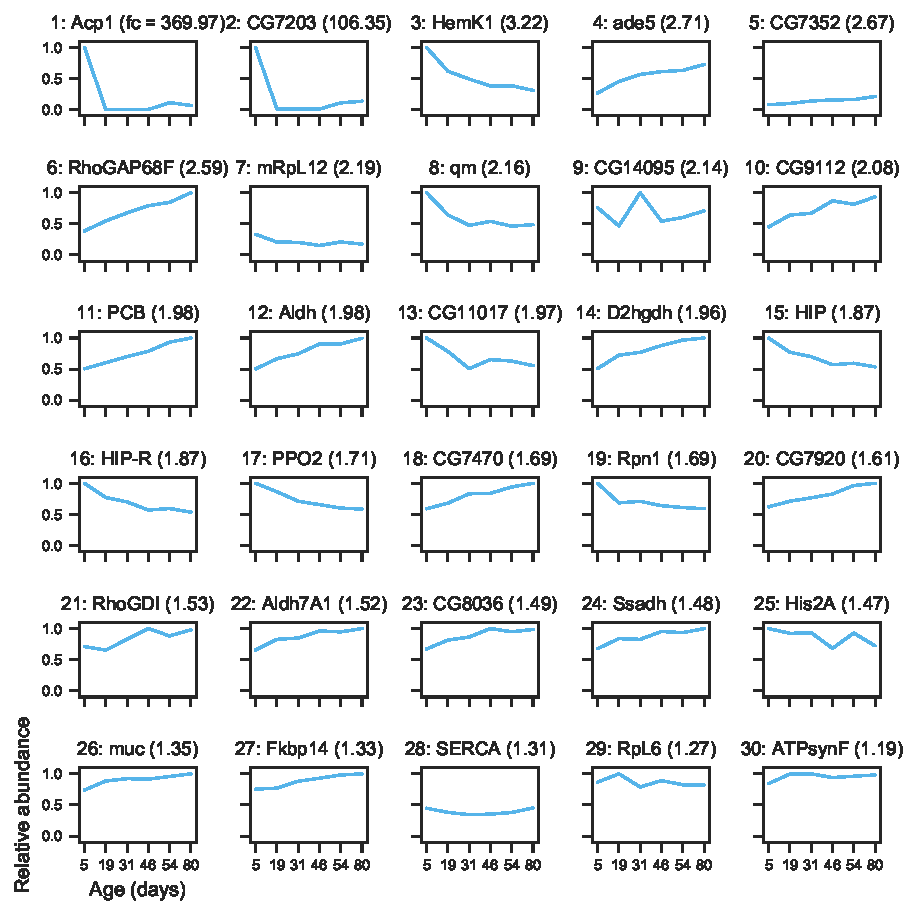
\includegraphics{./Chapter_fly/figS4}
%     \caption{%
%          Proteins specifically altered in ageing.
%          Profiles of significantly altered proteins in ageing are shown.
%          Maximum abundances are scaled to 1.
%          Numbers in parentheses denote the maximum observed fold change (fc).
%          Proteins are sorted in descending order of maximum observed fold change.
%     }
%     \label{fig:fly-figS4}
% \end{figure}

%(\ref{fig:fly-figS5})
To understand the dynamics of protein alterations following Aβ42 induction,
we clustered the profiles of proteins significantly altered in Aβ42 flies using
a Gaussian mixture model (\ref{fig:fly-fig2}c).
The proteins clustered best into four sets, determined by the BIC,
which was smallest with four clusters.
In comparison to healthy flies, cluster 1 contains proteins that have
consistently higher abundance in Aβ42 flies.
Conversely, cluster 2 contains proteins that have lower abundance in Aβ42 flies.
The abundances of proteins from clusters 1 and 2 are affected from the onset
of disease at day $5$, and remain at similar levels as the disease progresses.
Proteins in cluster $3$ follow a similar trend in healthy and Aβ42 flies
and increase in abundance with age.
However, cluster 4 proteins decrease in abundance as the disease progresses,
whilst remaining steady in healthy flies.

% \begin{figure}[!hbt]
%     \centering
%     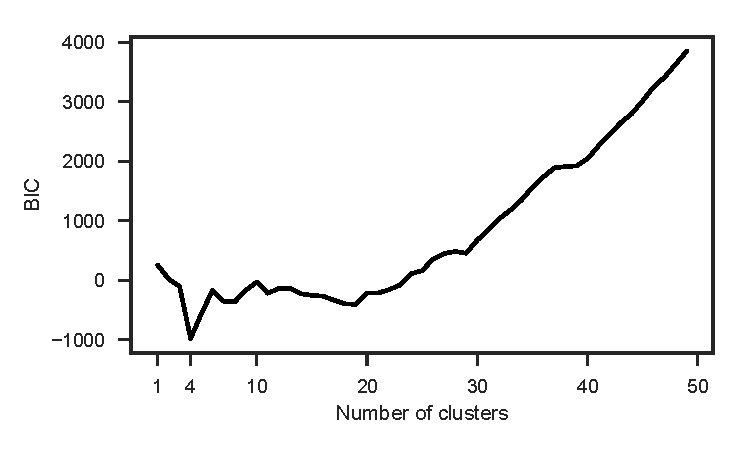
\includegraphics[width=0.6\textwidth]{./Chapter_fly/figS5}
%     \caption{%
%         Model selection for clustering of the significantly altered proteins using
%         a Gaussian mixture model.
%         The best model was chosen using the Bayesian information criterion (BIC),
%         which penalises complex models.
%     }
%     \label{fig:fly-figS5}
% \end{figure}

We performed a statistical GO enrichment analysis on each cluster,
but found no enrichment of terms.
Furthermore, we also saw no enrichment when we analysed all $228$ proteins together.

\subsection{Brain proteins significantly altered by Aβ42 have distinct network properties}

% (\ref{fig:fly-figS6}
%; Supplementary Data 4)
Following the analyses of brain proteome dysregulation in Aβ42 flies,
we analysed the $228$ significantly altered proteins in the context of the
brain protein interaction network to determine whether their network properties
are significantly different to the other brain proteins.
We used a subgraph of the STRING \cite{Szklarczyk2015} network
induced on the \num{3093} proteins identified by IM-DIA-MS
(see \ref{sec:fly-networks-methods} for more details).
This subgraph contained $183$ of the $228$ significantly altered proteins.
We then calculated four graph theoretic network properties (\ref{fig:fly-fig3}a)
of these $183$ significantly altered proteins contained in this network:

\begin{itemize}
    \item degree, the number of edges that a node has,
    \item shortest path, the smallest node set that connect any two nodes
    \item largest connected component, the largest node set for which all nodes have at least one edge to any of the other nodes;
    \item betweenness centrality, the proportion of all shortest paths in the network that a particular node lies on
\end{itemize}

% \begin{figure}[!hbt]
%     \centering
%     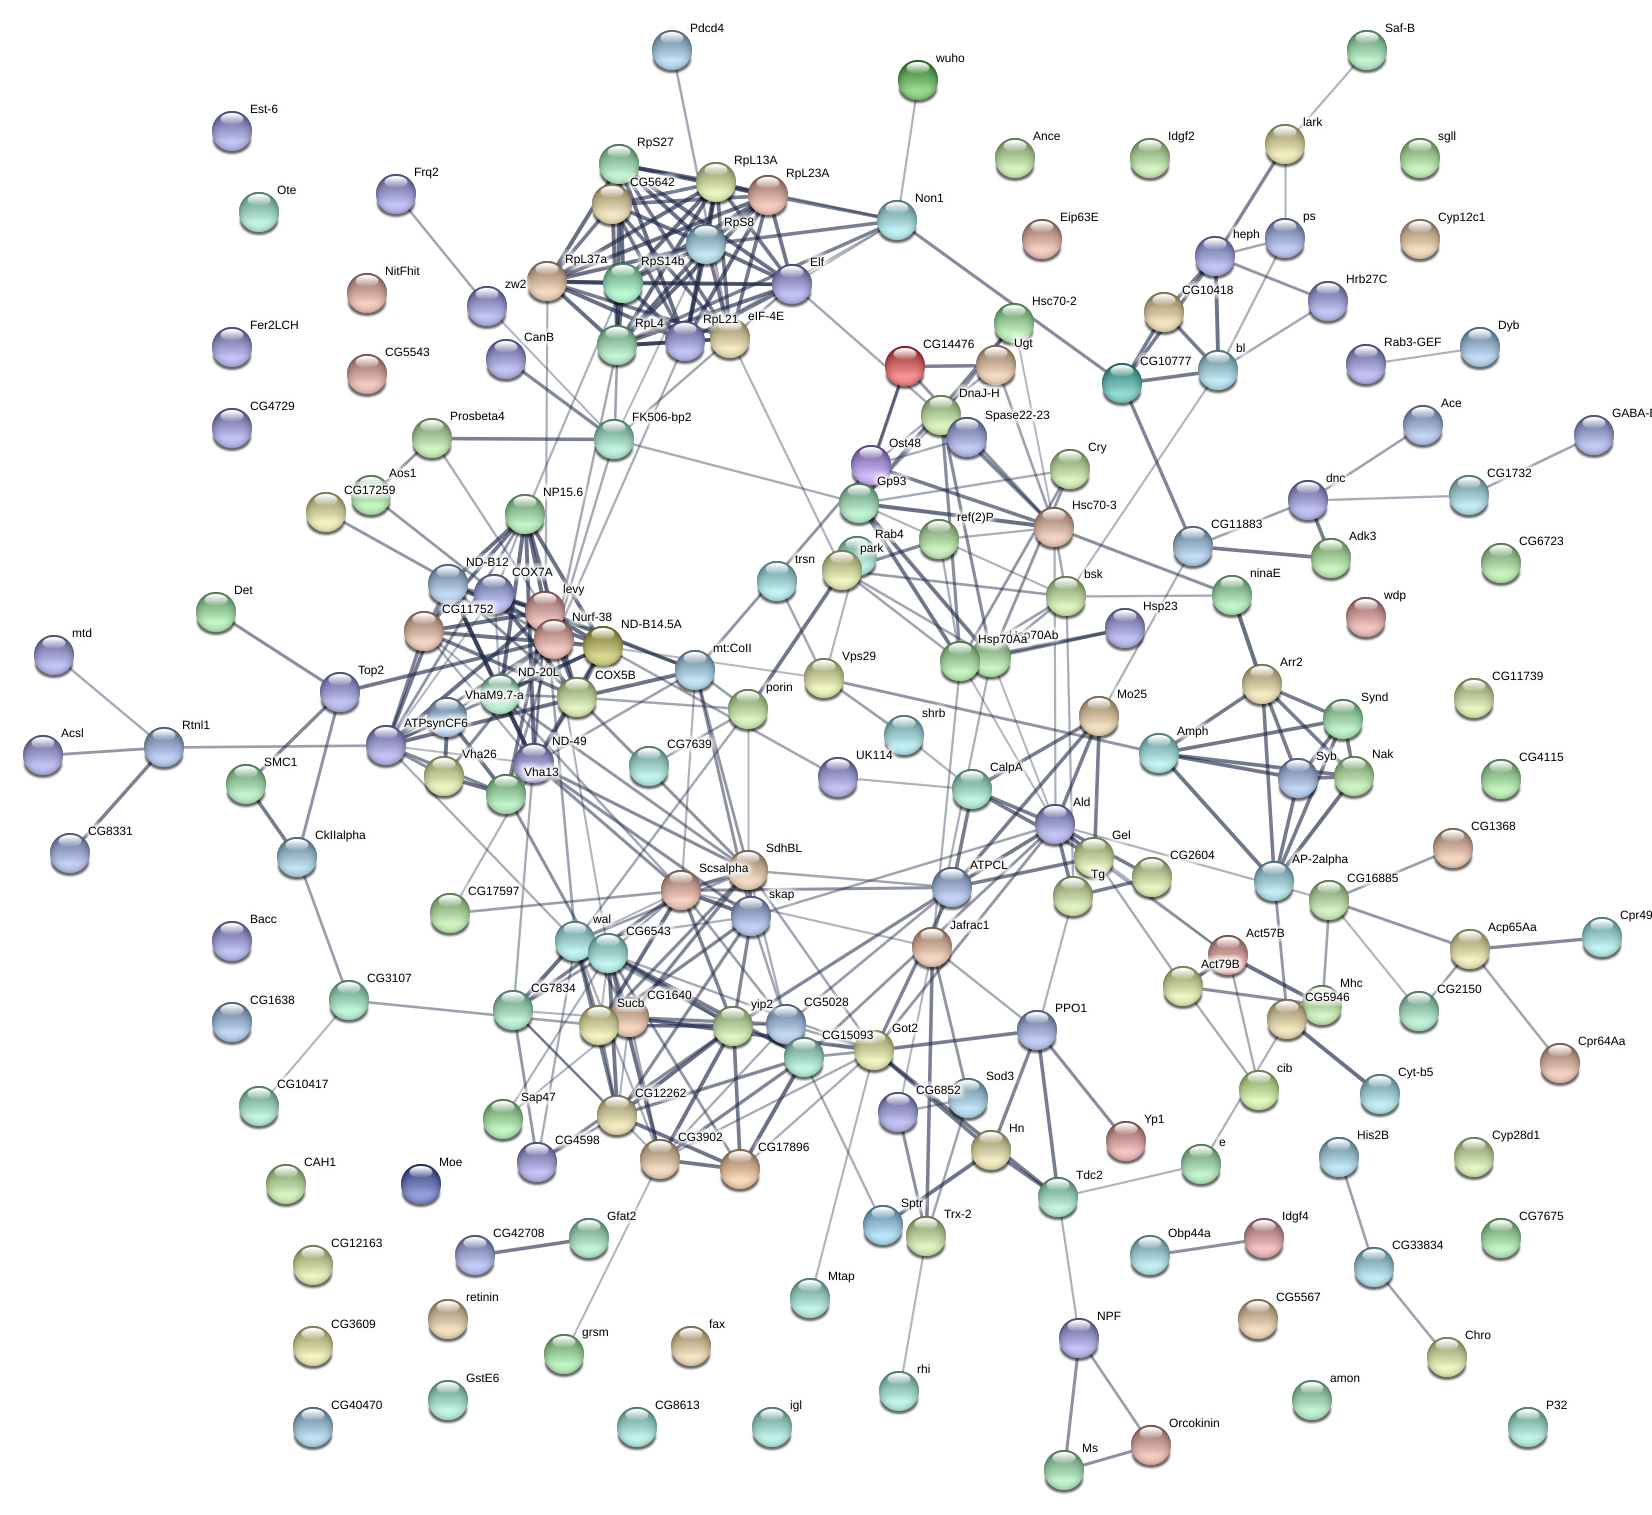
\includegraphics{./Chapter_fly/figS6}
%     \caption{%
%         Interactions of the 183 significantly altered proteins present in the STRING network.
%         A subgraph of the STRING network was induced on the 3093 proteins identified by
%         IM-DIA-MS in healthy or Aβ42 flies and the largest connected component was selected
%         (2428 nodes and 44,561 edges).
%         The subgraph contained 183 of the 228 significantly altered proteins
%         (
%         %Supplementary Data 3
%         ).
%         Edges are weighted by their interaction strength in the STRING database and
%         edges with `combined score' weight $< 0.5$ have been removed from the network.
%     }
%     \label{fig:fly-figS6}
% \end{figure}

\begin{figure}[!hbt]
    \centering
    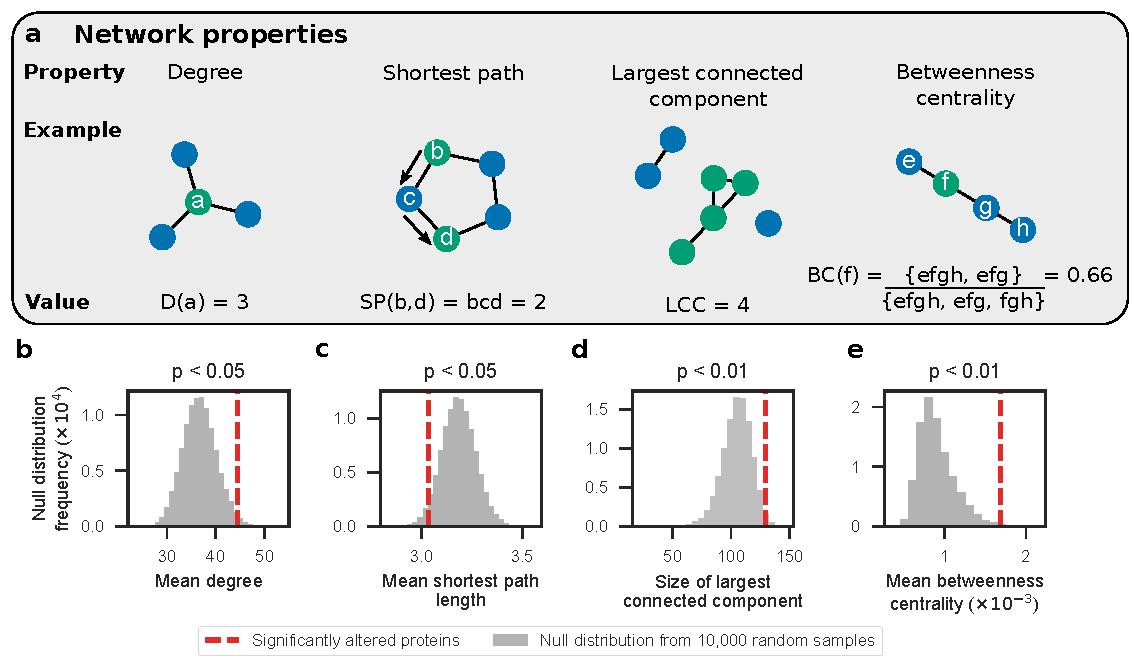
\includegraphics[width=\textwidth]{./Chapter_fly/fig3}
    \caption{%
        Significantly altered proteins have statistically significant network properties
        in the brain protein interaction network.
        (a) Network properties that were calculated:
        degree, the number of edges that a node has;
        shortest path, the smallest node set that connect any two nodes;
        largest connected component, the largest node set for which all nodes have at least
        one edge to any of the other nodes;
        and betweenness centrality, the proportion of all shortest paths in the network
        that a particular node lies on.
        Using a subgraph of the STRING network induced on the \num{3093} proteins identified by
        IM-DIA-MS in healthy and Aβ42 flies, the significance of four network
        characteristics were calculated for the $183$ significantly altered proteins
        contained in this subgraph.
        (b) mean degree;
        (c) mean shortest path length between a node and the remaining $182$ nodes;
        (d) the size of the largest connected component in the subgraph induced on these nodes;
        and (e) mean betweenness centrality.
        One-sided non-parametric $P$ values were calculated using null distributions of the
        test statistics, simulated by randomly sampling $183$ nodes from the network \num{10000} times.
    }
    \label{fig:fly-fig3}
\end{figure}

We performed hypothesis tests and found that these proteins have statistically significant
network properties.
Firstly, the significantly altered proteins make more interactions than expected
(mean degree $P < 0.05$; \ref{fig:fly-fig3}b).
Therefore, these proteins may further imbalance the proteome by disrupting the expression
or activity of proteins they interact with.
Secondly, not only are these proteins close to each other
(mean shortest path $P < 0.05$; \ref{fig:fly-fig3}c),
but also $129$ of them form a connected component
(size of largest connected component $P < 0.01$; \ref{fig:fly-fig3}d).
These two pieces of evidence suggest that Aβ42 disrupts proteins at the centre of the proteome.
Lastly, these proteins lie along shortest paths between many pairs of nodes
(mean betweenness centrality $P < 0.01$; \ref{fig:fly-fig3}e)
and may control how signals are transmitted in cells.
Proteins with high betweenness centrality are also more likely to be essential genes
for viability \cite{Yu2007}.
Taken together, these findings suggest that the proteins significantly altered in AD are
important in the protein interaction network.

\subsection{Predicting the severity of Aβ42-induced protein alterations using network properties}

We predicted how severely particular Aβ42-associated protein alterations may affect
the brain using two network properties—the tendency of a node to be a hub or a bottleneck.
In networks, nodes with high degree are hubs for communication,
whereas nodes with high betweenness centrality are bottlenecks that regulate how signals
propagate through the network.
Protein expression tends to be highly correlated to that of its neighbours in the
protein interaction network.
One exception to this rule, however, are bottleneck proteins,
whose expression tends to be poorly correlated with that of its neighbours \cite{Yu2007}.
This suggests that the proteome is finely balanced and that the expression of
bottleneck proteins is tightly regulated to maintain homeostasis.
We analysed the hub and bottleneck properties of the significantly altered proteins and
identified four hub-bottlenecks and five nonhub-bottlenecks that correlate with
Aβ42 expression (\ref{fig:fly-fig4}a) and analysed how their abundances change during normal ageing and
as pathology progresses (\ref{fig:fly-fig4}b).

\begin{figure}[!hbt]
    \centering
    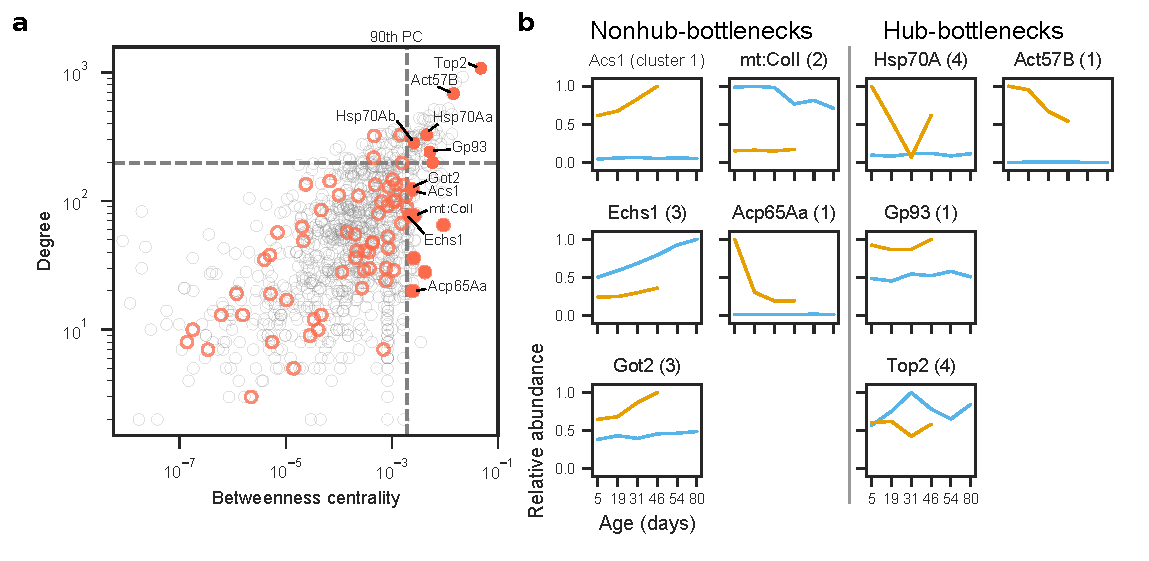
\includegraphics[width=1.05\textwidth]{./Chapter_fly/fig4}
    \caption{%
        Analysis of hubs and bottlenecks in the brain protein interaction network.
        In networks, nodes with high degree are hubs and nodes with high
        betweenness centrality are bottlenecks.
        (a) Degree (hub-ness) is plotted against betweenness centrality (bottleneck-ness)
        in the brain protein interaction network for all proteins identified by
        IM-DIA-MS (grey circles).
        Of the significantly altered proteins (red circles),
        hub-bottleneck ($>$ \nth{90} percentile (PC) for degree and betweenness centrality) and
        nonhub-bottleneck proteins ($>$ \nth{90} PC for betweenness centrality) are highlighted
        (filled red circles).
        (b) Profiles of significantly altered bottleneck proteins implicated in Aβ42 toxicity.
        Maximum abundances are scaled to unity.
        Numbers in parentheses denote which cluster from \ref{fig:fly-fig2}c the protein was in.
    }
    \label{fig:fly-fig4}
\end{figure}

Non-hub bottleneck proteins (\ref{fig:fly-fig4}b) Acs1 and Got2 levels were
stably expressed throughout normal ageing in our healthy flies but increased upon
Aβ42 induction and continued to rise with age in Aβ42 flies.
On the other hand, Echs1 abundance increased in healthy flies during normal ageing,
but its levels were reduced upon Aβ42 induction and its ageing-dependent increase
was diminished in Aβ42 flies compared to controls.
Levels of mt:CoII (a COX subunit) declined with age in healthy control,
but not in Aβ42, fly brain, although its expression was downregulated compared to
controls at all time-points following Aβ42 induction.
Finally, the cuticle protein Acp65Aa was also upregulated in Aβ42 flies compared to controls,
but levels fell sharply between $5$ and $19$ days of age.

Of the four hub-bottlenecks (\ref{fig:fly-fig4}b) Hsp70A was significantly upregulated
at early time-points ($5$ days) in Aβ42 flies, dropped between days $5$ and $31$ post-induction,
then increased at later time-points, compared to healthy controls
which exhibited stable expression of this protein throughout life.
We found that Gp93 was increased across age in Aβ42 flies compared to controls,
possibly suggesting an early and sustained protective mechanism against Aβ42-induced damage.
DNA topoisomerase 2 (Top2), an essential enzyme for DNA double-strand break repair,
was decreased in Aβ42 flies, following a pattern which mirrors changes in its expression
with normal ageing.
Finally, we found that actin (Act57B) was increased in Aβ42 flies but declined with age,
in comparison to control fly brains which displayed stable expression across life.

Due to the importance of these hub and bottleneck proteins in the protein interaction network,
we predict that AD-associated alterations in their abundance will likely have a
significant effect on the cellular dynamics of the brain.

\subsection{Dysregulated proteins are associated with known AD and ageing network modules}

%, Supplementary Data 5
% The smallest module (MCODE module 8) is shown in
% % \ref{fig:fly-figS7}
% .
%, Supplementary Data 6
Finally, we clustered the protein interaction network into modules and performed a
GO enrichment analysis on modules that contained any of the
$228$ significantly altered proteins.
We saw no GO term enrichment when we tested these proteins clustered
according to their abundance profiles (\ref{fig:fly-fig2}c),
presumably because the proteins affected in AD are diverse and involved in many
different biological processes.
However, by testing network modules for functional enrichment,
we exploited the principle that interacting proteins are functionally associated.
Using a subgraph of the STRING network containing the significantly altered proteins
and their directly-interacting neighbours (\ref{sec:fly-networks-methods}),
we used MCODE \cite{Bader2003} to find modules of densely interconnected nodes.
We chose to include neighbouring proteins to compensate for proteins that may not
have been detected in the MS experiments due to the stochastic nature of observing
peptides and the wide dynamic range of biological samples \cite{Lazar2016a}.
The resulting subgraph contained \num{4842} proteins,
including $183$ of the $228$ significantly altered proteins,
as well as $477$ proteins that were only identified in healthy or Aβ42 flies
and \num{3125} proteins that were not identified in our IM-DIA-MS experiments.

$12$ modules were present in the network (\ref{fig:fly-fig5}a).
Module sizes range from $302$ nodes to $17$ nodes.
The proportion of these modules that were composed of significantly altered proteins
ranged from \numrange{0}{8}$\%$.
All but one of the modules were enriched for processes implicated in AD and ageing
(\ref{fig:fly-fig5}), including respiration and
oxidative phosphorylation, transcription and translation, proteolysis,
DNA replication and repair, and cell cycle regulation.
These modules contained two proteins that were recently found to be significantly altered
in the brain of AD mice \cite{Savas2017} and are both upregulated four-fold in AD:
adenylate kinase, an adenine nucleotide phosphotransferase, and the armadillo protein Arm,
involved in creating long-term memories.
ApoB was found in the second highest scoring module that contains proteins involved
in translation and glucose transport \cite{Niccoli2016} (\ref{fig:fly-fig5}).

\begin{figure}[!hbt]
    \centering
    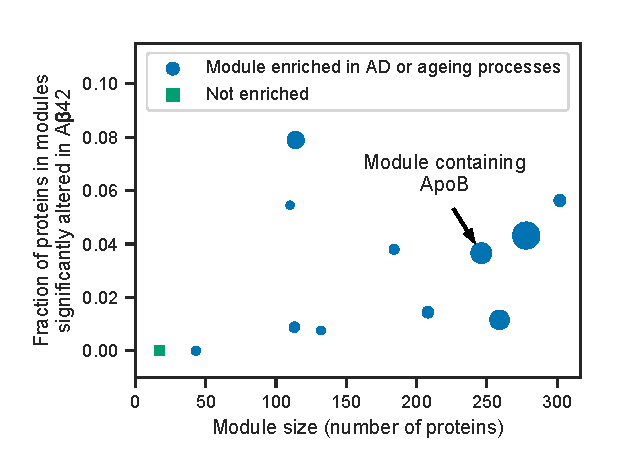
\includegraphics{./Chapter_fly/fig5}
    \caption{%
        Analysis of network modules enriched for AD or ageing processes.
        MCODE was used to identify network modules in a subgraph of the STRING network
        containing the significantly altered proteins and their directly-interacting neighbours.
        The size of the resulting $12$ modules is plotted against the fraction of proteins
        in these modules that are significantly altered in AD.
        Module 2 is annotated as containing ApoB.
        Marker sizes denote the MCODE score for the module.
    }
    \label{fig:fly-fig5}
\end{figure}

% \begin{figure}[!hbt]
%     \centering
%     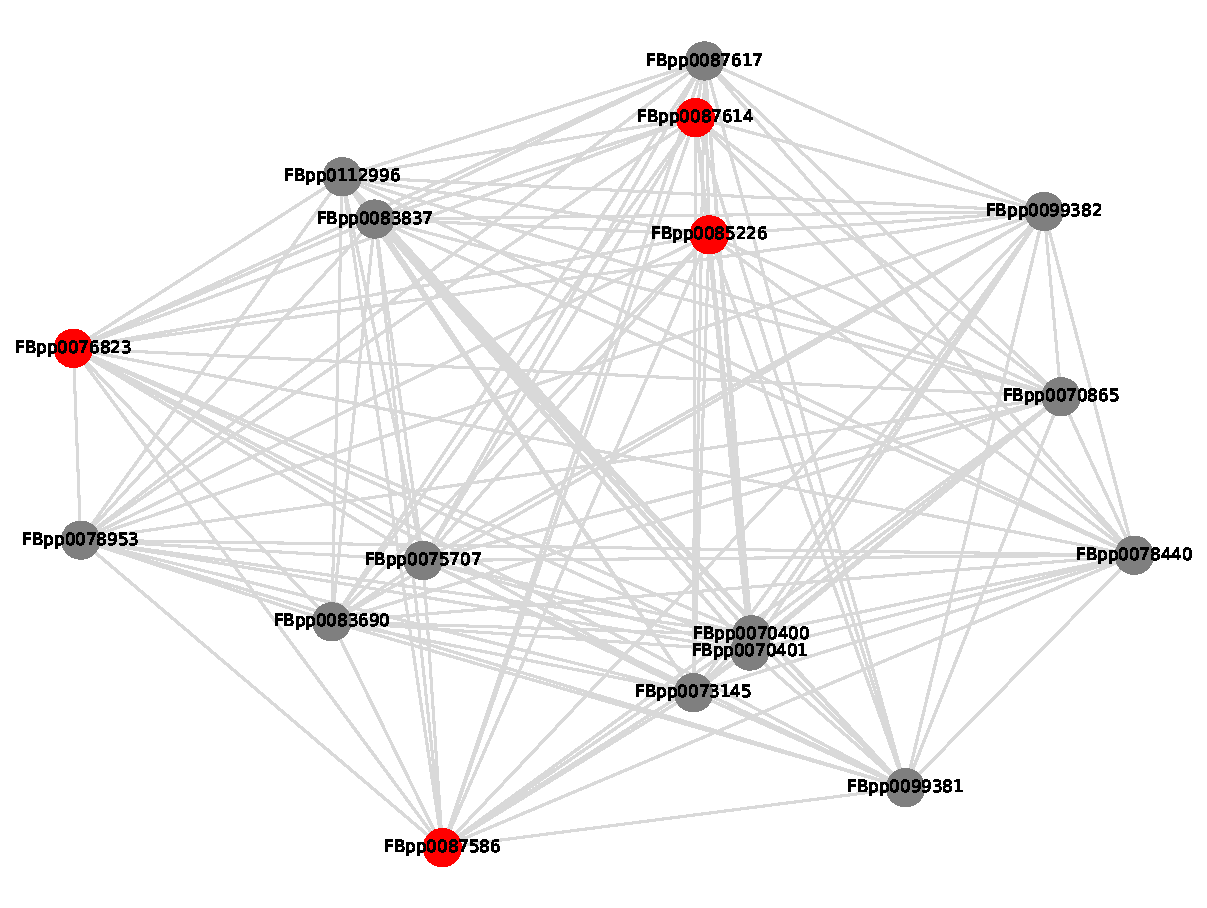
\includegraphics{./Chapter_fly/figS7}
%     \caption{%
%         Network diagram of MCODE module.
%         Using a subgraph of the STRING network containing the significantly altered
%         proteins and their directly-interacting neighbours,
%         we used MCODE to find modules of densely interconnected nodes.
%         We chose to include neighbouring proteins to compensate for proteins that
%         may not have been detected in the MS experiments due to the stochastic nature of
%         observing peptides and the wide dynamic range of biological samples.
%         The resulting subgraph contained 4842 proteins,
%         including 183 of the 228 significantly altered proteins,
%         as well as 477 proteins that were only identified in healthy or Aβ42 flies and
%         3125 proteins that were not identified in our IM-DIA-MS experiments.
%         12 modules were present in the network.
%         This figure details the interactions between proteins in the smallest module
%         % (module 8 in Supplementary Data 5).
%         .
%         Red nodes denote proteins that are significantly altered in Aβ42 flies.
%     }
%     \label{fig:fly-figS7}
% \end{figure}

In humans, the greatest genetic risk factor for AD is the $\epsilon$4 allele of ApoE---an
apolipoprotein involved in cholesterol transport and repairing brain injuries \cite{Liu2013b}.
A recent study showed that ApoE is only upregulated in regions of the mouse brain
that have increased levels of Aβ \cite{Savas2017},
indicating a direct link between the two proteins.
Although flies lack a homolog of ApoE, they do possess a homolog of the related
apolipoprotein ApoB (Apolpp) \cite{Palm2012}, which contributes to AD in mice \cite{Bereczki2008,Loffler2013}
and is correlated with AD in humans \cite{Caramelli1999,Zhang2004}.
Interestingly, whilst it was not identified by IM-DIA-MS,
ApoB interacts with $12$ significantly altered proteins in the STRING network,
so is included in the subgraph induced on the significantly altered proteins
and their neighbours.
ApoB was found in the second highest scoring module that contains proteins involved in
translation and glucose transport \cite{Niccoli2016} (\ref{fig:fly-fig5}).

% (Supplementary Data 3).
% (Supplementary Data 7)
We analysed the $31$ proteins significantly altered in normal ageing,
but not AD.
Of the $29$ proteins that were contained in the STRING network,
$24$ interact directly with at least one of the AD significantly altered proteins,
suggesting an interplay between ageing and AD at the pathway level.
Using a subgraph of the STRING network induced on these proteins and their \num{1603} neighbours,
we identified eight network modules
that were enriched for
ageing processes \cite{Lopez-Otin2013}, including respiration, unfolded protein and
oxidative damage stress responses, cell cycle regulation, DNA damage repair, and apoptosis.

\section{Discussion}
\label{discussion}

Despite the substantial research effort spent on finding drugs against AD,
effective treatments remain elusive.
We need to better understand the molecular processes that govern the onset and progression
of the complex pathologies observed in this condition to AD.
This knowledge will help to identify new drug targets to treat and prevent AD.

\subsection{AD models capture the temporal effects of AD}

Analysis of post-mortem human brain tissue is an important way to study dementia,
but cannot capture the progression of pathology from the initiation of disease.
Due to their short lifespan and ease of genetic manipulation, model organisms
such as \textit{Drosophila melanogaster} provide a tractable system in which to examine the
progression of AD pathology across life.
We performed a longitudinal study of the \textit{Drosophila} brain proteome,
using an inducible model of AD, label-free quantitative IM-DIA-MS and network analyses.
We were able to track alterations in protein levels from the point of exposure to human
Aβ42 and the widespread interaction of Aβ42 with brain signalling networks as
pathology progresses.

\subsection{The brain proteome becomes dysregulated with age, in the absence of AD}

We identified $61$ proteins which were significantly altered with age in fly brain,
$31$ of which were not altered in response to Aβ42.
Of these, structural chitin proteins (Acp1 and CG7203),
mitochondrial associated proteins (HemK1 and mRPL12),
geranylgeranyl transferases (qm), and proteostasis proteins (HIP, HIP-R and Rpn1)
were significantly downregulated with age.
Indeed, loss of mitochondrial function and proteostasis are key features of the ageing
brain \cite{Hou2019} in agreement with these observations.
Recent studies also suggest a role for geranylgeranyl transferase I-mediated protein
prenylation in mediating synaptogenesis and learning and memory \cite{Afshordel2014,Gao2016}.
Our findings suggest that this may represent a novel mechanism of regulation
and maintenance of these functions during ageing, which warrants further investigation.

Proteins involved in inositol monophosphate (IMP) biosynthesis (ade5),
endosome recycling (RhoGAP68F and RhoGDI), oxidation-reduction processes
(D2hgdh, Aldh and Aldh7A1), pyruvate metabolism (PCB and muc),
neurotransmitter function (Ssadh) and ER-related protein folding (FKBP14)
were increased with age in fly brain in our study.
Oxidative damage is a key feature of ageing brain and loss of aldehyde dehydrogenase
(Aldh) function, which detoxifies oxidative stress inducing aldehydes,
has been shown to be associated with promoting age-related neurodegeneration
and cognitive dysfunction in mice \cite{DSouza2015,Ohsawa2008}.
Phosphatidylinositol signalling is important for stabilising mood and behaviour,
and IMP inhibition is thought to partially mediate the beneficial effects of lithium
in the treatment of bipolar disorder \cite{Sade2016}.

Rho GTPases are involved in maintenance of synaptic function \cite{Afshordel2014},
and reductions in their levels correlate with ageing and increases in their expression
with foraging behaviour in the brain of honey bees \cite{Dobrin2012}.
Our finding that inhibitors of these enzymes (Rho GAPs and Rho GDIs) are upregulated
in ageing fly brain further suggests that changes in their activity may mediate loss of
synaptic function throughout life.

Ageing is also characterised by a progressive loss of metabolic function,
and studies suggest that ATP-generating metabolites, such as pyruvate,
improve cognitive function \cite{Owen2011} as reflected by upregulation of
pyruvate carboxylase and muc, a component of the pyruvate dehydrogenase complex,
in our data set.

Finally, several proteins fluctuated in expression across age in our flies,
including those involved in DNA repair (His2A), protein translation (RpL6),
and ER calcium homeostasis (SERCA), processes which have been previously reported in
association with brain ageing \cite{Maynard2015,Anisimova2018,Mattson2018}.
Although alterations in these proteins are independent of Aβ42 expression in our flies,
further work is required to investigate their functional role in preserving brain function
with age and their potential to increase the vulnerability of the ageing brain
to neurodegenerative diseases.

\subsection{AD is associated with widespread dysregulation of the brain proteome}

Our proteomic analyses identified Aβ42-induced alterations in levels of $228$ proteins,
which clustered into four groups.
First, those which were either elevated (cluster 1) or reduced (cluster 2) in AD
relative to controls throughout life, and dysregulation of which may initiate
AD pathogenesis, be involved in early stages of disease progression, or represent
defense mechanisms that could be harnessed for protection.
Second, those which were altered in correlation with ageing in healthy and Aβ42 flies
(cluster 3).
Finally, those which changed in Aβ42 flies across life but independently of ageing-dependent
effects in healthy controls (cluster 4).
Further work is required to determine whether reduction of these proteins plays a causal role
in disease pathogenesis that could be targeted therapeutically,
or whether their decline represents a protective response to damage.

\subsection{Brain proteins significantly altered by Aβ42 have distinct network properties}

Moreover, computational analysis of these proteins revealed significant network properties
within the fly brain proteome.
Assessing hub and bottleneck properties, many of the Aβ42-induced proteomic changes
represented alterations in bottleneck proteins suggesting that they play key roles in
downstream cellular function.
Of these, some display non-hub properties indicating that they are important for
maintaining cellular homeostasis in a targeted fashion,
whereas others also displayed hub properties, suggesting that they are central
in linking cellular signalling pathways to maintain cell function.

\subsection{Proteins dysregulated in AD are hubs and bottlenecks in protein networks}

We identified five nonhub-bottleneck proteins and four hub-bottleneck proteins,
the expression of which was altered in Aβ42 flies relative to controls across life.
Due to the importance of these hub and bottleneck proteins in the protein interaction network,
we predict that AD-associated alterations in their abundance will likely have a
significant effect on the cellular dynamics of the brain.
Indeed, some of these proteins play key molecular roles in metabolism (AscI, Echs1, Got2),
protein homeostasis (Hsp70A, Gp93), protection against oxidative stress (mt:CoII),
and DNA damage (Top2).
These processes have been shown to affect neuronal function and protection
against proteo-toxicity.

Acyl-CoA synthetase long chain (Acs1), Enoyl-CoA hydratase, short chain 1 (Echs1),
and Aspartate aminotransferase (Got2), are metabolic enzymes with previous links to
neuronal function and damage \cite{Cai2011,Szutowicz2013}.
Got2 produces the neurotransmitter L-glutamate from aspartate,
is involved in assembly of synapses and becomes elevated following brain injury \cite{Maas1977}.

Cytochrome c oxidase (COX), complex IV of the mitochondrial electron transport chain,
uses energy from reducing molecular oxygen to water to generate a proton gradient across
the inner mitochondrial membrane.
Although Aβ is known to inhibit COX activity \cite{Casley2002},
the link between COX and AD is unclear.
In AD patients, COX activity---but not abundance---is reduced,
resulting in increased levels of ROS \cite{Cardoso2004}.
However, in COX-deficient mouse models of AD,
plaque deposition and oxidative damage are reduced \cite{Fukui2007}.

Hsp70A is a heat shock protein that responds to hypoxia and Gp93 is a stress response
protein that binds unfolded proteins,
consistent with responses to abnormal Aβ42 aggregation in our flies.

DNA topoisomerase 2 (Top2) is an essential enzyme for DNA double-strand break repair.
Double-strand breaks occur naturally in the brain as a consequence of neuronal activity---an
effect that is aggravated by Aβ \cite{Suberbielle2013}.
As a consequence of deficient DNA repair machinery,
deleterious genetic lesions may accumulate in the brain and exacerbate neuronal loss.

The cuticle protein Acp65Aa is a chitin,
this class of which have been detected in AD brains and suggested to facilitate Aβ
nucleation \cite{Castellani2005}.

Finally, actin (Act57B) is a structural protein, and depolymerisation of F-actin
filaments in a mouse AD model before onset of AD pathology \cite{Kommaddi2018}.
Alterations in these proteins may represent either adaptive responses to the presence
of abnormal protein aggregates, such as Aβ42, or mediators of neuronal toxicity.
Further functional genomic studies are therefore required to establish the causal role
of these processes in governing onset and progression of AD pathology.

Assessing the human orthologs of these genes, identified using DIOPT \cite{Hu2011a},
indicates that several of these bottleneck proteins have been previously implicated
in association with AD or other neurological conditions in humans
or mammalian models of disease.
ACSL4 (Acs1 ortholog) has been shown to associate with synaptic growth cone development
and mental retardation \cite{Meloni2002}.
Mutations in ECHS1 (Echs1 ortholog), an enzyme involved in mitochondrial fatty acid oxidation,
associate with Leigh Syndrome, a severe developmental neurological disorder \cite{Peters2014}.
Proteomic studies have revealed that GOT2 (Got2 ortholog) is down-regulated
in infarct regions following stroke \cite{Datta2013},
and in AD patient brain \cite{McKenzie2017}.
Integrating data from human post-mortem brain studies,
HSPA1A (Hsp70Aa ortholog) upregulates in the protein interaction network of AD patients
compared to healthy controls \cite{Chi2016},
and has recently been suggested to block APP processing
and Aβ production in mouse brain \cite{Gerber2019}.
Synthetic, fibrillar, Aβ42 reduces expression of TOP2B (Top2 ortholog)
in rat cerebellar granule cells and in a human mesenchymal cell line,
suggesting this may contribute to DNA damage in response to amyloid \cite{Terzioglu-Usak2017}.
HSP90B1 (Gp93 ortholog) shows increased expression following TBI in mice \cite{Tzekov2016},
and associates with animal models of Huntington’s disease \cite{MatthiasE2015}.
Finally, ACTB (Act57B ortholog) has been implicated as a significant AD risk gene
and central hub node using integrated network analyses across GWAS \cite{Talwar2014}.

\subsubsection{Nonhub-bottlenecks: Acs1, Echs1, Got2, mt:CoII and Acp65Aa}

Three of the nonhub-bottlenecks, Acyl-CoA synthetase long chain (Acs1), Enoyl-CoA hydratase,
short chain 1 (Echs1), and Aspartate aminotransferase (Got2),
are metabolic enzymes with previous links to neuronal function and damage.
Acs1 and Echs1 are involved in the production of acetyl-CoA from fatty acids.
Many enzymes involved in acetyl-CoA metabolism associate with AD leading to
acetyl-CoA deficits in the brain and loss of cholinergic neurons \cite{Szutowicz2013}.
Got2 produces the neurotransmitter L-glutamate from aspartate,
is involved in assembly of synapses and becomes elevated following brain injury \cite{Maas1977}.
Brain Acs1 and Got2 levels were stably expressed throughout normal ageing in our healthy
flies but increased upon Aβ42 induction and continued to rise with age in Aβ42 flies.
This suggests that levels of these proteins increase independently of ageing in AD,
but correlate closely with disease progression.
On the other hand, Echs1 abundance increases in healthy flies during normal ageing,
but its levels were reduced upon Aβ42 induction and its ageing-dependent increase
was diminished in Aβ42 flies compared to controls.
This may reflect a protective response with ageing that is suppressed by Aβ42 toxicity.

Cytochrome c oxidase (COX), complex IV of the mitochondrial electron transport chain,
uses energy from reducing molecular oxygen to water to generate a proton gradient across
the inner mitochondrial membrane.
Levels of mt:CoII (a COX subunit) declined in aged healthy control fly brain.
mt:CoII expression was downregulated in Aβ42 flies compared to controls at all time-points
and was stably-expressed across age following Aβ42 induction.
The link between COX and AD is unclear, although Aβ is known to inhibit COX activity \cite{Casley2002}.
For example, in AD patients, COX activity—but not abundance—is reduced,
resulting in increased levels of ROS \cite{Cardoso2004}.
However, in COX-deficient mouse models of AD, plaque deposition and
oxidative damage are reduced \cite{Fukui2007}.
Hence, the ageing-dependent decline in mt:CoII may represent either a reduction
in COX function which renders the brain vulnerable to damage and is exacerbated
by Aβ42 toxicity, or a protective mechanism against both ageing and amyloid toxicity.

The cuticle protein Acp65Aa was also upregulated in Aβ42 flies,
but levels fell sharply between $5$ and $19$ days.
However, it is surprising that we identified Acp65Aa in our samples,
as it is not expected to be expressed in the brain.
One explanation may involve chitin,
which has been detected in AD brains and has been suggested to facilitate Aβ nucleation \cite{Castellani2005}.
Amyloid aggregation has previously been shown to plateau around $15$ days post-induction \cite{Rogers2012},
which is around the same time that Acp65Aa drops in Aβ42 flies.
Our results suggest that Aβ42 causes an increase in Acp65Aa expression early in the disease,
but further experiments are needed to confirm this and to investigate its relationship
with nucleation and the aggregation process.

\subsubsection{Hub-bottlenecks: Hsp70A, Gp93, Top2 and Act75B}

The four hub-bottlenecks are consistent with Aβ42 inducing stress.
Hsp70A, a heat shock protein that responds to hypoxia, was significantly upregulated
at early time-points ($5$ days) in Aβ42 flies, compared to healthy controls
which exhibited stable expression of this protein throughout life.
Although the levels dropped in Aβ42 flies between days $5$ and $31$ post-induction,
at later time-points Hsp70A increased again, possibly suggesting a two-phase response to
hypoxia in Aβ42 flies.
We found that Gp93—a stress response protein that binds unfolded proteins—to be increased
across age in Aβ42 flies compared to controls possibly suggesting an early and sustained
protective mechanism against Aβ42-induced damage.
DNA topoisomerase 2 (Top2), an essential enzyme for DNA double-strand break repair,
was decreased in Aβ42 flies, following a pattern which mirrors changes in its expression
with normal ageing.
Double-strand breaks occur naturally in the brain as a consequence of neuronal
activity---an effect that is aggravated by Aβ \cite{Suberbielle2013}.
As a consequence of deficient DNA repair machinery,
deleterious genetic lesions may accumulate in the brain and exacerbate neuronal loss.

Finally, we found that actin (Act57B) was increased in Aβ42 flies,
in agreement with two recent studies on mice brains \cite{Savas2017,Kommaddi2018}.
Kommaddi and colleagues found that Aβ causes depolymerisation of F-actin filaments
in a mouse AD model before onset of AD pathology \cite{Kommaddi2018}.
The authors showed that although the concentration of monomeric G-actin increases,
the total concentration of actin remains unchanged.
It has long been known that G-, but not F-,
actin is susceptible to cleavage by trypsin \cite{Jacobson1976},
permitting its detection and quantification by IM-DIA-MS.
Hence, the apparent increase of actin in Aβ42 flies may be due to F-actin depolymerisation,
which increases the pool of trypsin-digestible G-actin, and is consistent with the findings
of Kommaddi et al.
To confirm whether total actin levels remain the same in the brains of Aβ42 flies,
additional experiments would have to be carried out in the future,
for example tryptic digestion in the presence of MgADP---which makes F-actin susceptible to
cleavage \cite{Hozumi1988}---and transcriptomic analysis of actin mRNA.
Furthermore, actin polymerisation is ATP-dependent, so increased levels of G-actin
may indicate reduced intracellular ATP.
In addition, ATP is important for correct protein folding and therefore reduced levels may
lead to increased protein aggregation in AD.

ACSL4, ECHS1, and HSP90B1 have no reported association with AD or related dementias,
however, which suggests that our study has the potential to identify new targets
in the molecular pathogenesis of this disease.
Our study also provides additional information about the homeostasis of these proteins
across life from the point of amyloid production.
For example, the abundances of Acs1 and Got2 are elevated following Aβ42 induction
and continue to increase with age relative to controls.
Echs1 is reduced in Aβ42 flies compared to controls but increases across life
in parallel with ageing-dependent increases in this protein.
Structural proteins Acp65Aa and Act57B are elevated in response to Aβ42,
but decline across life whilst remaining stable in control flies.
Gp93 and Top2 are either elevated or reduced in response to Aβ42 but mirror
ageing-dependent alterations in their expression.
mt:CoII is reduced following Aβ42 expression at all time-points,
but reduced with ageing in controls.
Hsp70A is increased early in Aβ42 flies, reduced to control levels in mid-life,
then elevated at late pathological stages whilst remaining stable in healthy controls.

\subsection{Dysregulated proteins are associated with known AD and ageing network modules}

Analysing GO enrichment using network modules,
to capture the diverse biological processes modified in AD,
we identified $12$ modules enriched for processes previously implicated in ageing and AD.
This validates the use of our \textit{Drosophila} model in identifying progressive molecular changes
in response to Aβ42 that are likely to correlate with progression of cognitive decline
in human disease.
Further work is required to modify the genes identified in our study at different ages,
in order to elucidate whether they represent mediators of toxicity as the disease progresses,
factors which increase neuronal susceptibility to disease with age
or compensatory protective mechanisms.
Model organisms will be essential in unravelling these complex interactions.
Our study therefore forms a basis for future analyses that may identify new targets
for disease intervention that are specific to age and/or pathological stage of AD.

\subsection{Conclusion}

To understand the dynamic molecular pathology of AD as the disease progresses, we carried out a longitudinal study of the brain proteome using an inducible \textit{Drosophila melanogaster} transgenic model of AD (TgAD) that expresses Arctic mutant Aβ42.
We were able to capture how Aβ42 toxicity affects the brain as the disease progresses in the AD brain.
We tracked alterations in the brain proteome from the point of amyloid induction, and across life.
We identified \num{3093} proteins using label-free quantitative ion-mobility data independent analysis mass spectrometry (IM-DIA-MS) \cite{Rodriguez-Suarez2013}, \num{1854} of which were common to healthy and Aβ42 flies.
Of these, we identified $228$ proteins that were significantly altered in AD, some of which overlapped with normal ageing but the majority of which were ageing-independent.
Proteins altered in response to Aβ42 were enriched for AD processes and have statistically significant network properties in the brain protein interaction network.
We also showed that these proteins are likely to be bottlenecks for signalling in the network, suggesting that they comprise important proteins for normal brain function.
Our data is a valuable resource to begin to understand the dynamic properties of Aβ42 proteo-toxicity during AD progression.
These data may also be useful for researchers to identify potential therapeutic candidates to treat AD at pre- and post-symptomatic stages.
Future functional studies will be required to determine the causal role of these proteins in mediating progression of AD using model organisms and to translate these findings to mammalian systems.

\section*{Addendum}

During the viva for this thesis, it was brought to our attention that some of the statistical methods
that we used to calculate differential gene expression were inappropriate for the type of data analysed in this project.
We chose the five methods that we used in this study because they can identify differentially expressed genes
in time-course data, albeit in microarray or RNA-Seq data, rather than quantitative mass spectrometry data.
The key issue here is that RNA-Seq data are count-based, so should be modelled using discrete distributions,
whereas, microarray data and quantitative mass spectrometry data are continuous, so should be modelled using
continuous distributions. Discrete data should not be modelled using continuous distributions and vice versa.

EDGE, limma and maSigPro were used appropriately in this study to model differential gene expression using
continuous distributions. However, DESeq2 and edgeR were inappropriate for these data, as these methods are
based on the (discrete) negative binomial distribution. Interestingly, edgeR, DESeq2 and limma detect similar proteins,
whereas, EDGE and maSigPro detect very different proteins (\ref{fig:fly-figS2}).

When we began this work, we were unable to find any methods designed to identify differentially expressed genes
in quantitative proteomics data. Subsequently, a number of methods have been developed, for example DEqMS \cite{Zhu2020a},
from the same group that developed DESeq and DESeq2, and DEP \cite{Zhang2018}, which is based on limma.

We thank the examiners for bringing this error to our attention.